% Created 2024-05-18 Sat 14:42
% Intended LaTeX compiler: pdflatex
\documentclass[aspectratio=169]{beamer}
\usepackage[utf8]{inputenc}
\usepackage[T1]{fontenc}
\usepackage{graphicx}
\usepackage{longtable}
\usepackage{wrapfig}
\usepackage{rotating}
\usepackage[normalem]{ulem}
\usepackage{amsmath}
\usepackage{amssymb}
\usepackage{capt-of}
\usepackage{hyperref}
\usepackage{appendixnumberbeamer}
\usepackage{amssymb}
\usepackage{tabularx}
\usepackage[group-separator={,}, group-minimum-digits=3]{siunitx}   % Format numbers
\usepackage[ruled]{algorithm2e}             % Algorithms
\usepackage{tikz}                           % Draw stuff
\usetikzlibrary{arrows.meta}                % Arrows for tikz
\usepackage{subcaption}                     % Subfigures
\usepackage{animate}                        % Created animated things
\usepackage{xcolor}
% Syntax: \colorboxed[<color model>]{<color specification>}{<math formula>}
\newcommand*{\colorboxed}{}
\def\colorboxed#1#{%
\colorboxedAux{#1}%
}
\newcommand*{\colorboxedAux}[3]{%
% #1: optional argument for color model
% #2: color specification
% #3: formula
\begingroup
\colorlet{cb@saved}{.}%
\color#1{#2}%
\boxed{%
\color{cb@saved}%
#3%
}%
\endgroup
}
\renewcommand{\arraystretch}{1.5}
\logo{
\begin{tikzpicture}[overlay,remember picture]
\node[left=0.2cm] at (current page.26){

\includegraphics[height=0.5cm]{img/u-state-black.png}
};
\end{tikzpicture}
}
\institute[USU] % (optional)
{
College of Engineering\\
Utah State University
}
\beamertemplatenavigationsymbolsempty
\addtobeamertemplate{navigation symbols}{}{%
\usebeamerfont{footline}%
\usebeamercolor[fg]{footline}%
\hspace{1em}%
\insertframenumber/\inserttotalframenumber
}
\newcommand\mycommfont[1]{\footnotesize\ttfamily\textcolor{gray}{#1}}
\newcommand{\T}{\mathcal{T}}                % To make it clear the difference
\newcommand{\Tau}{T}                        % between Tau and T
\newcommand{\AC}{AC(u, d, v, \eta)}         % Set the parameters for AC once
\newcommand{\UC}{UC(u, d, v)}               % Set the parameters for UC once
\newcommand{\ACi}{AC(u_i, d_i, q_i, \eta_i)}% Set the parameters for AC once
\newcommand{\UCi}{UC(u_i, d_i, q_i)}        % Set the parameters for UC once
\newcommand{\Not}{\textbf{not }}            % Custom `not' operator
\newcommand{\visit}{(i, b, a, e, u, d, q, \eta, \xi)}
\newcommand{\I}{\mathbb{I}}                 % Set of visit tuples
\newcommand{\C}{\mathbb{C}}                 % Charger availability information
\newcommand{\U}{\mathcal{U}}                % Uniform distribution
\newcommand{\W}{\mathcal{W}}                % Weighted distribution
\newcommand{\Sol}{\mathbb{S}}               % A shorthand for visit tuple
\newcommand{\M}{\mathbb{M}}                 % A shorthand for the metadata
\newcommand{\Hd}{\mathbb{H}}                % Set of discrete times
\newcommand{\Nu}{\mathcal{V}}               % Draw a nice Nu
\newcommand{\Iset}{I}                       % Set of visits 1-I
\newcommand{\Isetinit}{I_0}                 % Set of visits inital visits
\newcommand{\Isetfinal}{I_f}                % Set of visits final visits
\newcommand{\Bset}{B}                       % Set of visits 1-B
\newcommand{\Qset}{Q}                       % Set of visits 1-Q
\newcommand{\Jset}{J}                       % Set of visits 1-J
\newcommand{\Jsetq}{\mathbb{J}}             % Set of visits 1-J for queue active times
\newcommand{\Hset}{H}                       % Set of visits 1-H
\usetheme{default}
\usecolortheme{dolphin}
\author{Alexander Brown}
\date{\today}
\title{A POSITION ALLOCATION PROBLEM APPROACH TO THE BATTERY ELECTRIC BUS CHARGING PROBLEM}
\AtBeginSection[]{
\begin{frame}<beamer>\frametitle{Topic}\tableofcontents[currentsection]\end{frame}
\subsection{}
}
\hypersetup{
 pdfauthor={Alexander Brown},
 pdftitle={A POSITION ALLOCATION PROBLEM APPROACH TO THE BATTERY ELECTRIC BUS CHARGING PROBLEM},
 pdfkeywords={},
 pdfsubject={},
 pdfcreator={Emacs 29.3 (Org mode 9.6.15)}, 
 pdflang={English}}
\begin{document}

\maketitle
\begin{frame}{Outline}
\tableofcontents
\end{frame}


\section{Introduction}
\label{sec:org06d0a00}
\begin{frame}[label={sec:org6f27354}]{Problem Description}
\begin{columns}
\begin{column}{0.5\columnwidth}
\begin{center}
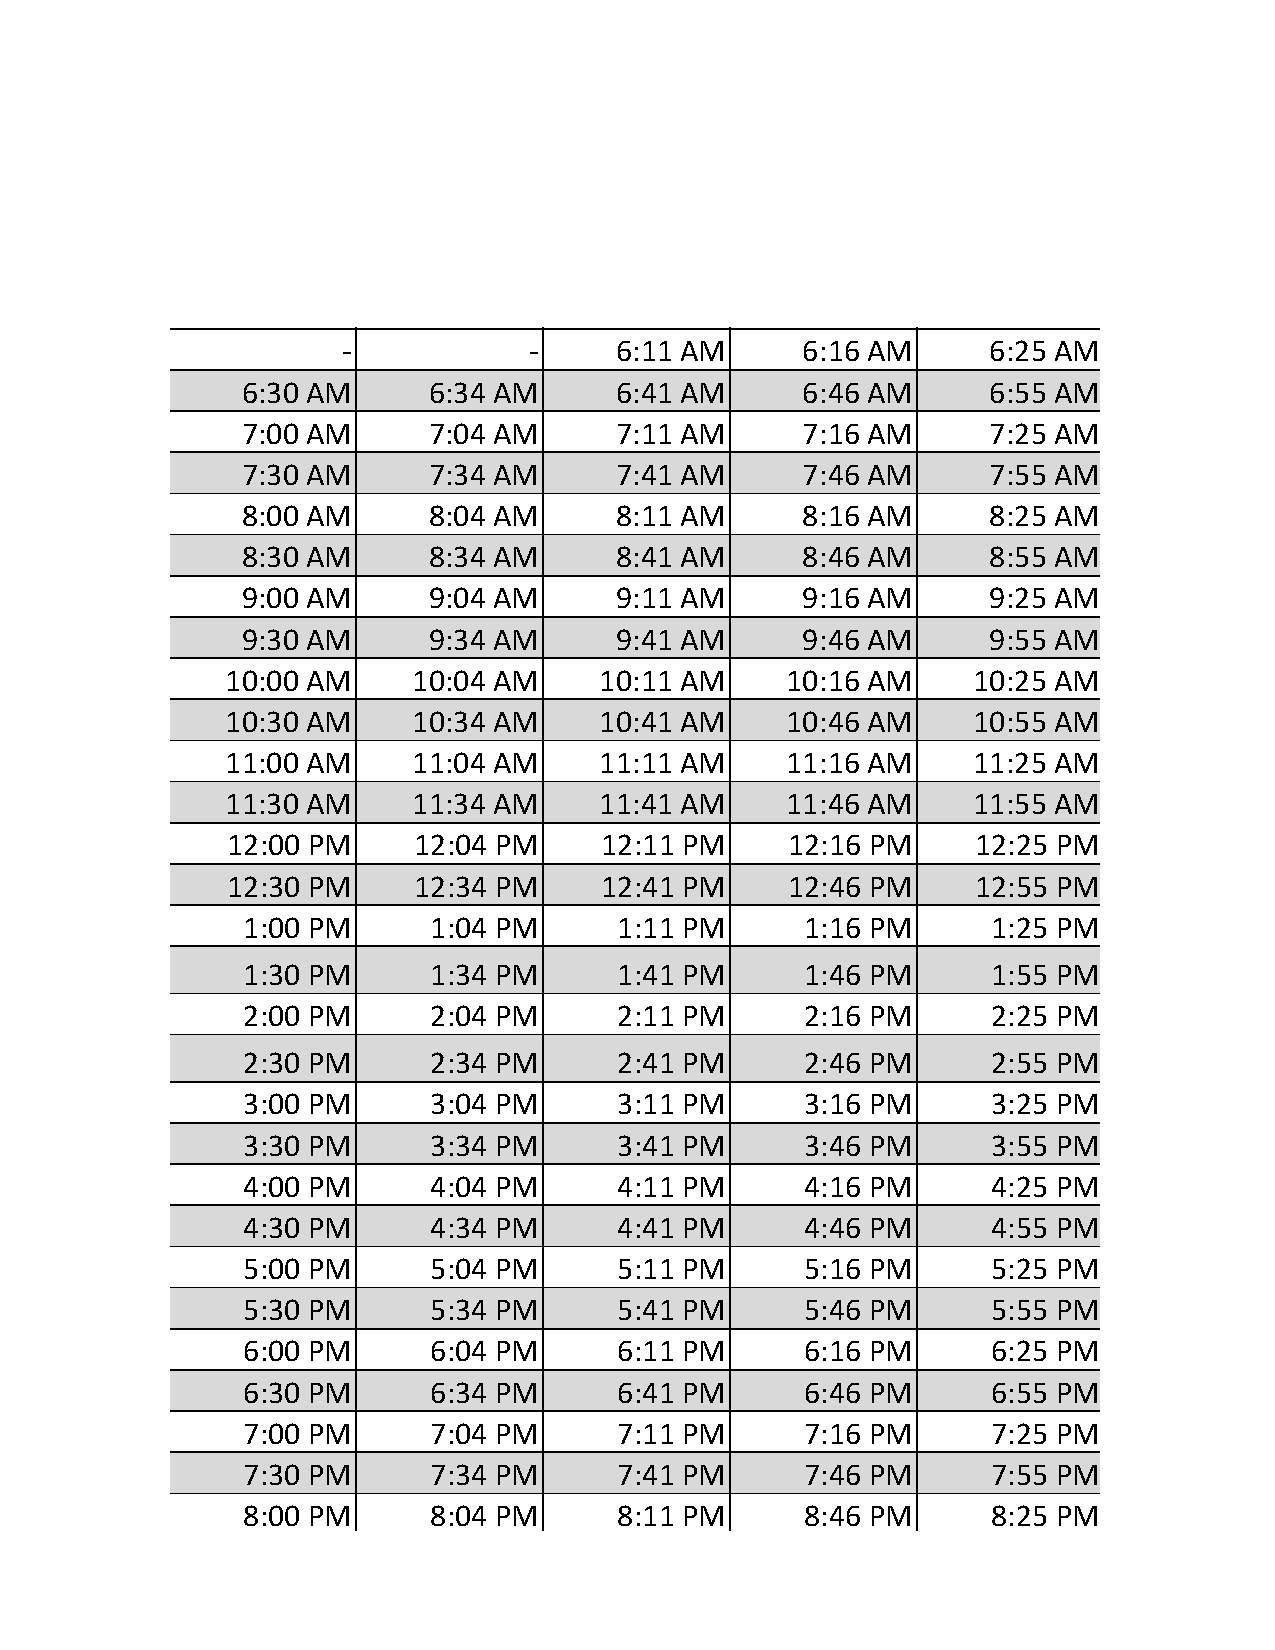
\includegraphics[width=0.8\textwidth]{./img/route-schedule.pdf}
\end{center}
\end{column}

\begin{column}{0.5\columnwidth}
\begin{figure}
    \centering
    \scalebox{0.4}{
      \centering
        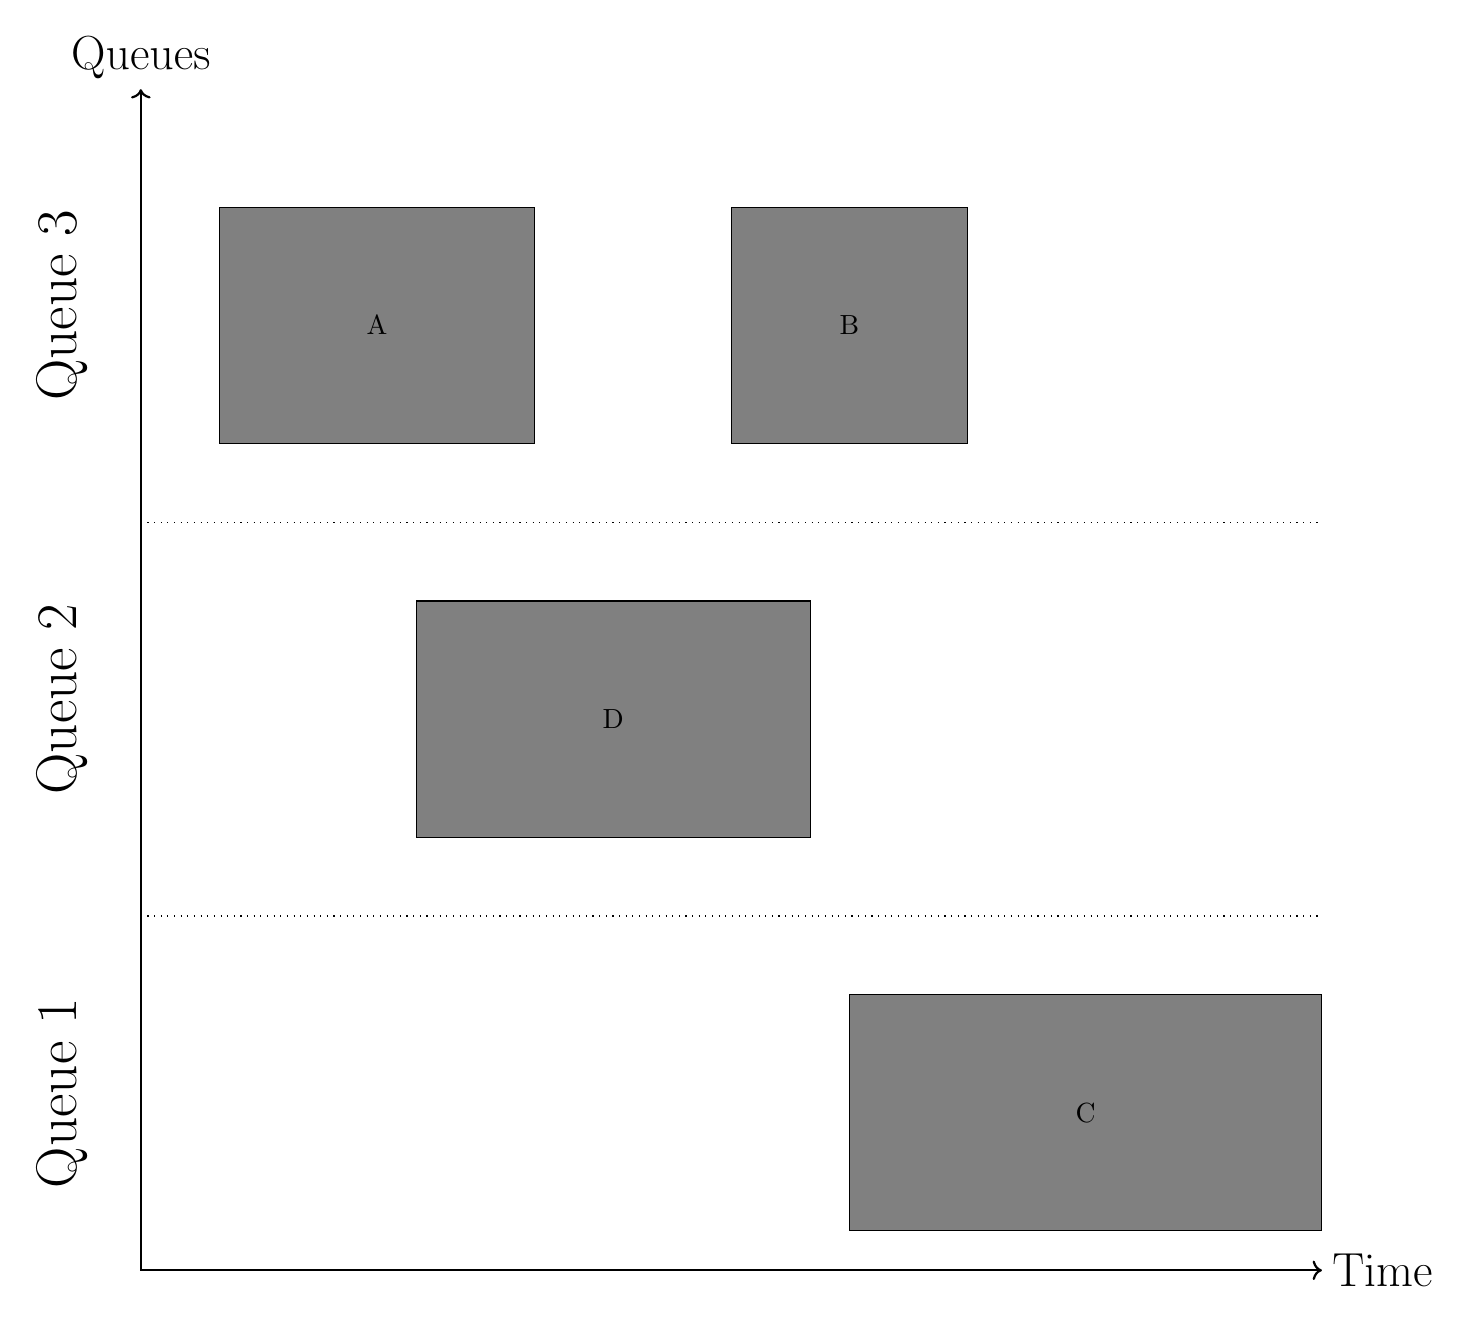
\begin{tikzpicture}
          % Variables
          \def \arrx   {2.0}
          \def \initx  {3.5}
          \def \endx   {8.5}
          \def \depx   {10.0}
          \def \yshift {5}

          % Axis
          \draw [thick,<->] (0,15) node[above]{\LARGE Queues} -- (0,0) -- (15,0) node[right]{\LARGE Time};

          % Rectangles
          \node[rectangle, draw, fill=gray, minimum width=4cm, minimum height = 3cm] at (3,12) {A};
          \node[rectangle, draw, fill=gray, minimum width=3cm, minimum height = 3cm] at (9,12) {B};
          \node[rectangle, draw, fill=gray, minimum width=5cm, minimum height = 3cm] at (6,7) {D};
          \node[rectangle, draw, fill=gray, minimum width=6cm, minimum height = 3cm] at (12,2) {C};

          % Y-axis labels
          \node[rotate=90] at (-1, 2.25) {\huge Queue 1};
          \node[rotate=90] at (-1, 7.25) {\huge Queue 2};
          \node[rotate=90] at (-1, 12.25) {\huge Queue 3};

          % Horizontal lines
          \draw[dotted] (0, 4.5) -- (15, 4.5);
          \draw[dotted] (0, 9.5) -- (15, 9.5);

        \end{tikzpicture}
      }
      \label{fig:spacial-and-temporal-constr}
\end{figure}
\end{column}
\end{columns}
\end{frame}

\begin{frame}[label={sec:org62e4d1f}]{Overall Objective}
\end{frame}
\begin{frame}[label={sec:orgb84f7f3}]{Model Objectives}
\end{frame}
\begin{frame}[label={sec:org2f3e303}]{Brief State Of The Art}
{\scriptsize
\begin{center}
\begin{tabularx}{\textwidth}{XXXXXXX}
\hline
Ref & Consumption & Demand & Linear & Non-linear & Charger Min. & Battery Health\\[0pt]
\hline
\cite{duan-2021-refor-mixed} & \(\checkmark\) &  & \(\checkmark\) &  &  & \\[0pt]
\cite{frendo-2021-open-sourc} & \(\checkmark\) & \(\checkmark\) & \(\checkmark\) &  &  & \\[0pt]
\cite{jahic-2019-preem} & \(\checkmark\) & \(\checkmark\) & \(\checkmark\) & \(\checkmark\) &  & \\[0pt]
\cite{mortensen-2023-cost-minim} & \(\checkmark\) & \(\checkmark\) & \(\checkmark\) &  &  & \\[0pt]
\cite{qin-2016-numer-analy} & \(\checkmark\) & \(\checkmark\) & \(\checkmark\) &  &  & \\[0pt]
\cite{rinaldi-2020-mixed-fleet} & \(\checkmark\) &  & \(\checkmark\) &  &  & \\[0pt]
\cite{whitaker-2023-a-network} & \(\checkmark\) &  &  & \(\checkmark\) & \(\checkmark\) & \(\checkmark\)\\[0pt]
\cite{zhou-2020-collab-optim} & \(\checkmark\) &  & \(\checkmark\) &  &  & \\[0pt]
\cite{zhou-2020-bi-objec} & \(\checkmark\) &  & \(\checkmark\) &  & \(\checkmark\) & \\[0pt]
BPAP & \(\checkmark\) &  & \(\checkmark\) &  & \(\checkmark\) & \(\checkmark\)\\[0pt]
SA BPAP & \(\checkmark\) & \(\checkmark\) & \(\checkmark\) & \(\checkmark\) & * & \(\checkmark\)\\[0pt]
\hline
\end{tabularx}
\end{center}
}
\end{frame}

\begin{frame}[label={sec:orgb3852eb}]{The Berth Allocation Problem\footnote{\url{https://www.mdpi.com/2077-1312/11/7/1280}}}
\begin{center}
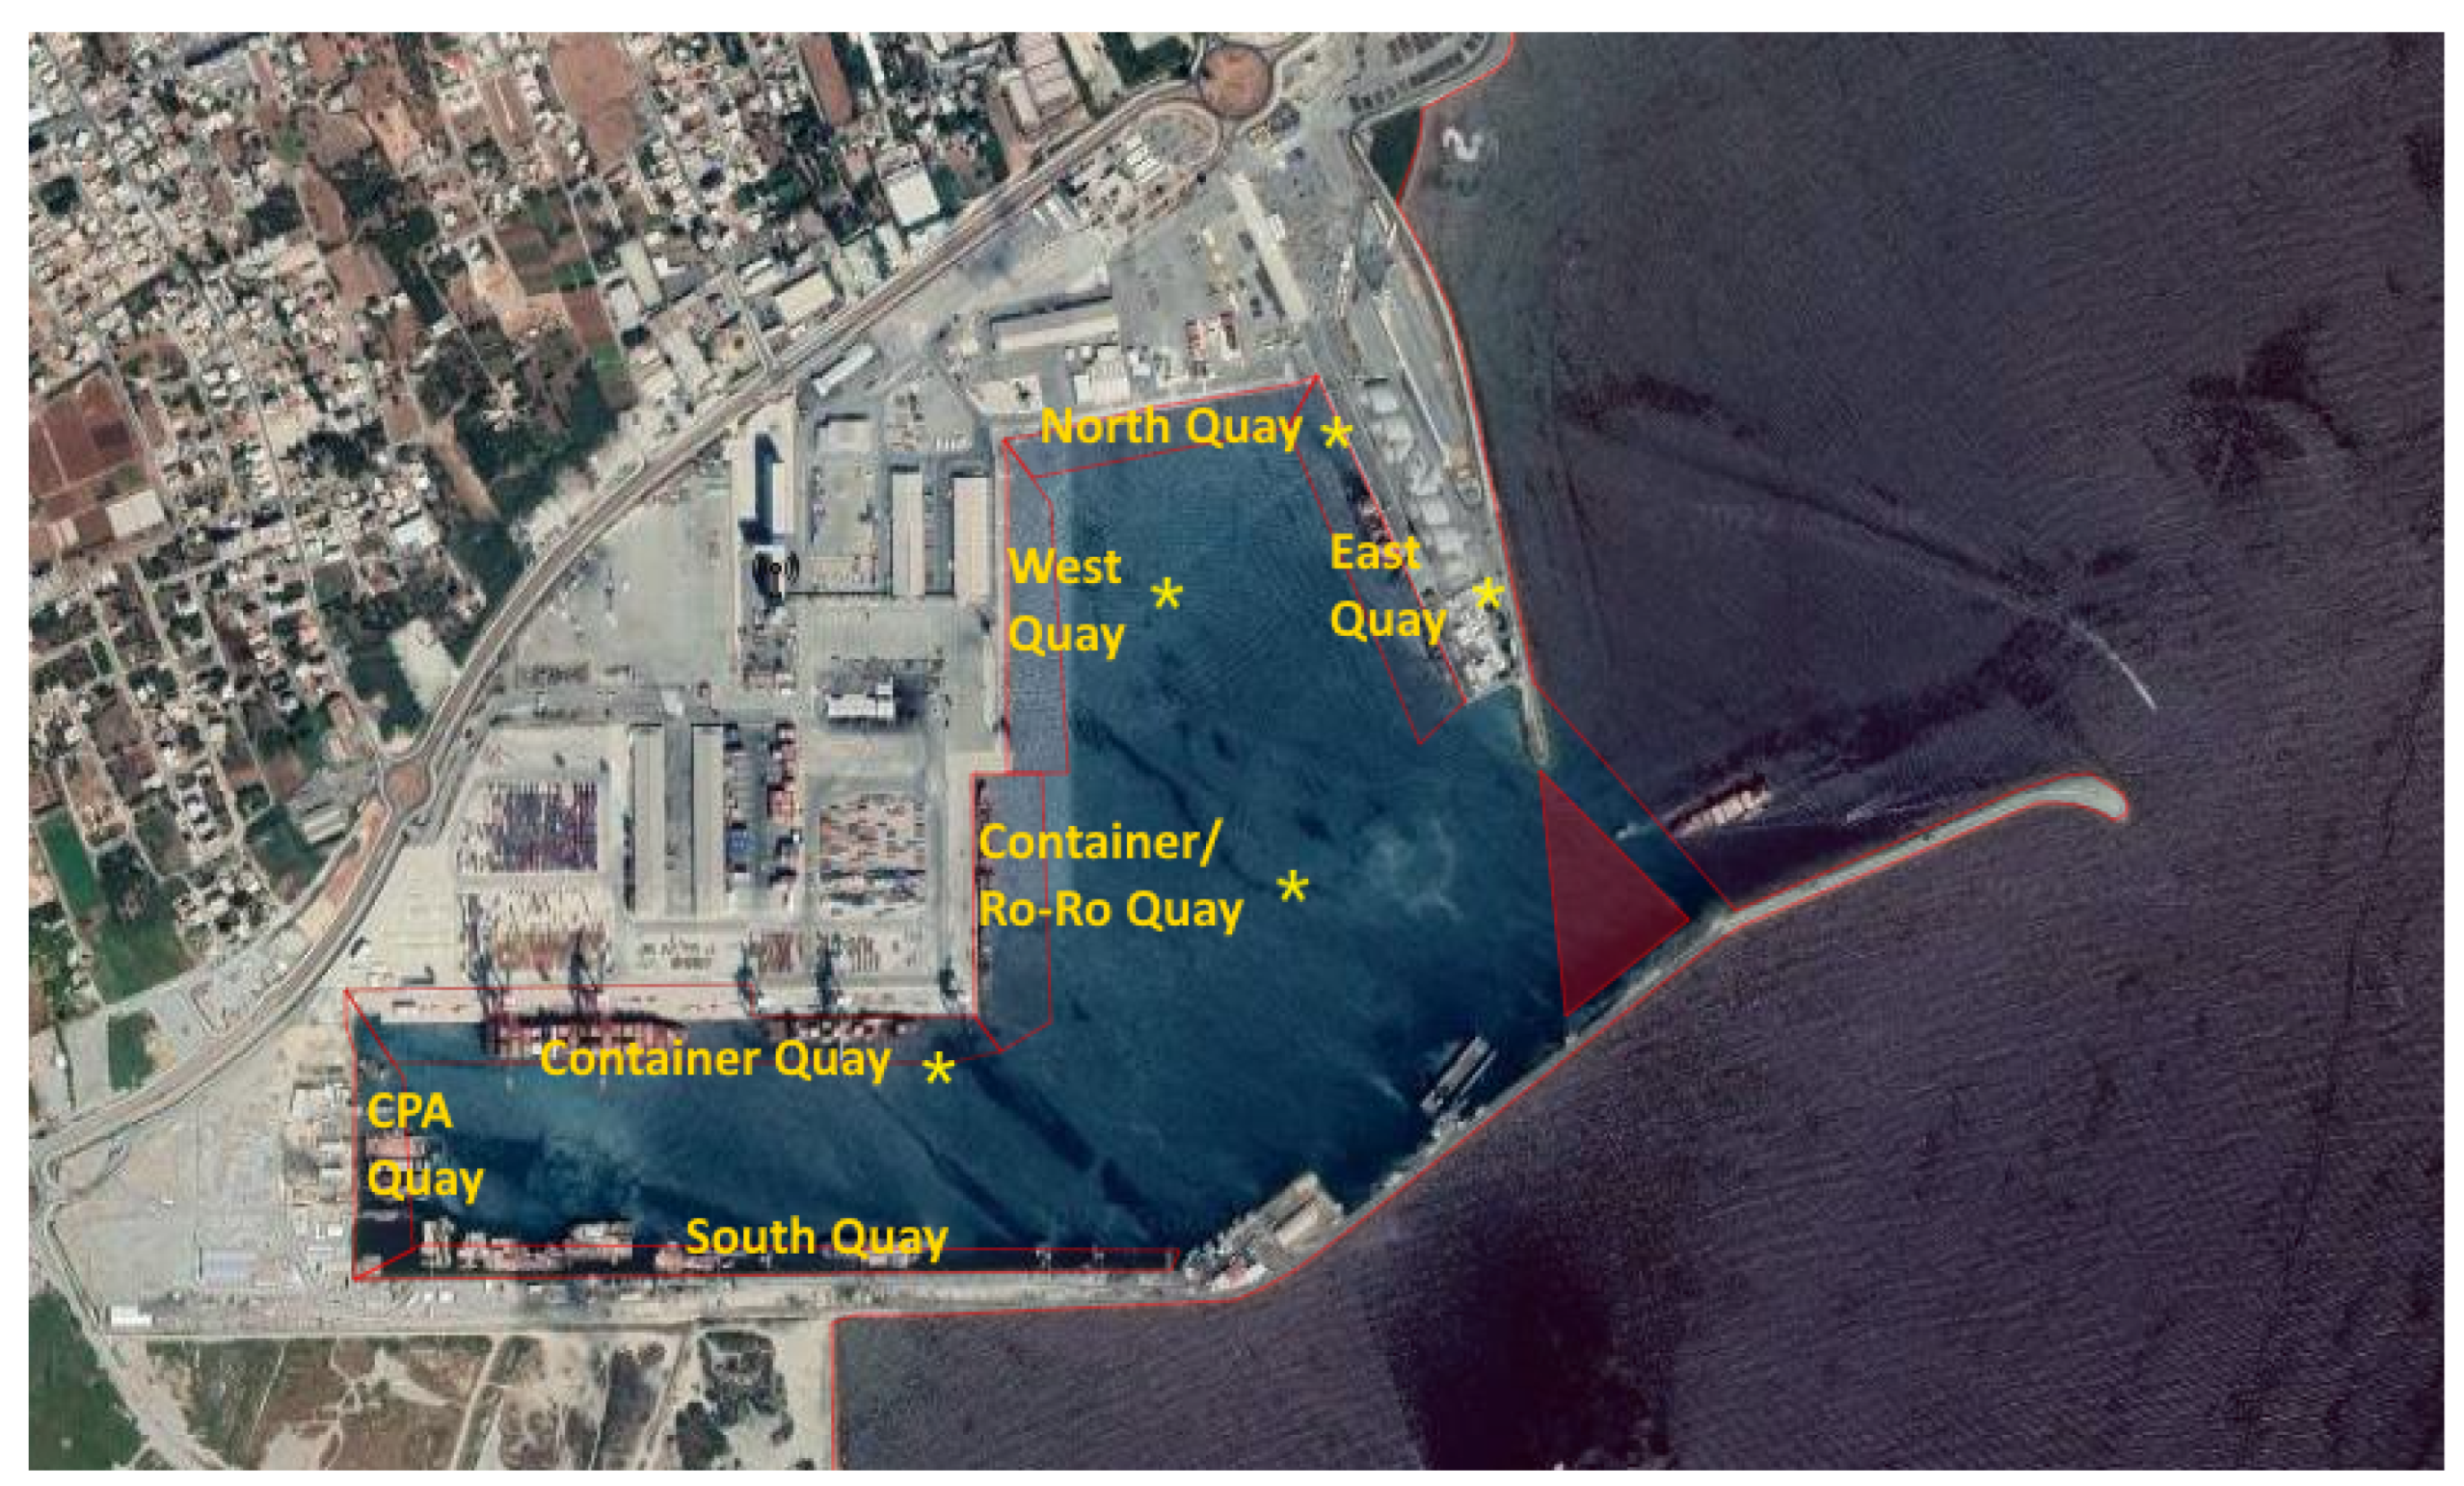
\includegraphics[width=0.8\textwidth]{./img/berthing-sky-picture.png}
\end{center}
\end{frame}

\begin{frame}[label={sec:orgdf37e4f}]{The Berth Allocation Problem}
\begin{columns}
\begin{column}{0.4\columnwidth}
\begin{itemize}
\item Vessels move down toward the quay
\item Receive service
\item Exit to the right
\end{itemize}

\noindent\rule{\textwidth}{0.5pt}
\begin{itemize}
\item A variant of the rectangle packing problem
\item Solves the problem of optimally assigning incoming vessels to be serviced
\end{itemize}
\end{column}

\begin{column}{0.6\columnwidth}
\begin{center}
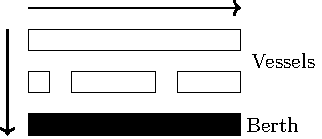
\includegraphics[width=0.6\textwidth]{./img/bap.pdf}
\end{center}

\begin{center}
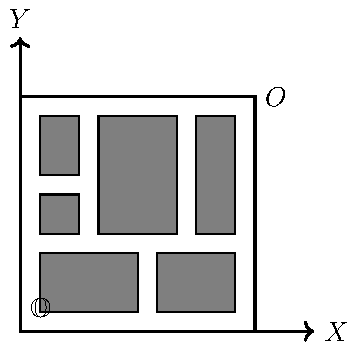
\includegraphics[width=0.5\textwidth]{./img/spatiotemporal-packing.pdf}
\end{center}
\end{column}
\end{columns}
\end{frame}

\begin{frame}[label={sec:orgd250729}]{The Position Allocation Problem}
\begin{columns}
\begin{column}{0.5\columnwidth}
{\begin{center} {\small \underline{PAP Behavior}}}\end{center}

{\small
\begin{itemize}
\item Service flow is left to right
\item Single charger type
\item All arrivals are considered unique
\item Service times are assumed to be known
\end{itemize}
}

\noindent\rule{\textwidth}{0.5pt}

{\begin{center} {\small \underline{Desired Behavior}}}\end{center}

{\small
\begin{itemize}
\item Discrete charger queues
\item Multiple charger types
\item Bus can have multiple visits
\item Propagate battery SOC across visits
\item Unknown charge times
\end{itemize}
}
\end{column}

\begin{column}{0.5\columnwidth}
\begin{center}
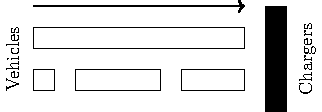
\includegraphics[width=0.7\textwidth]{./img/pap.pdf}
\end{center}

\begin{figure}
  \centering
  \scalebox{0.3}{
    \centering
    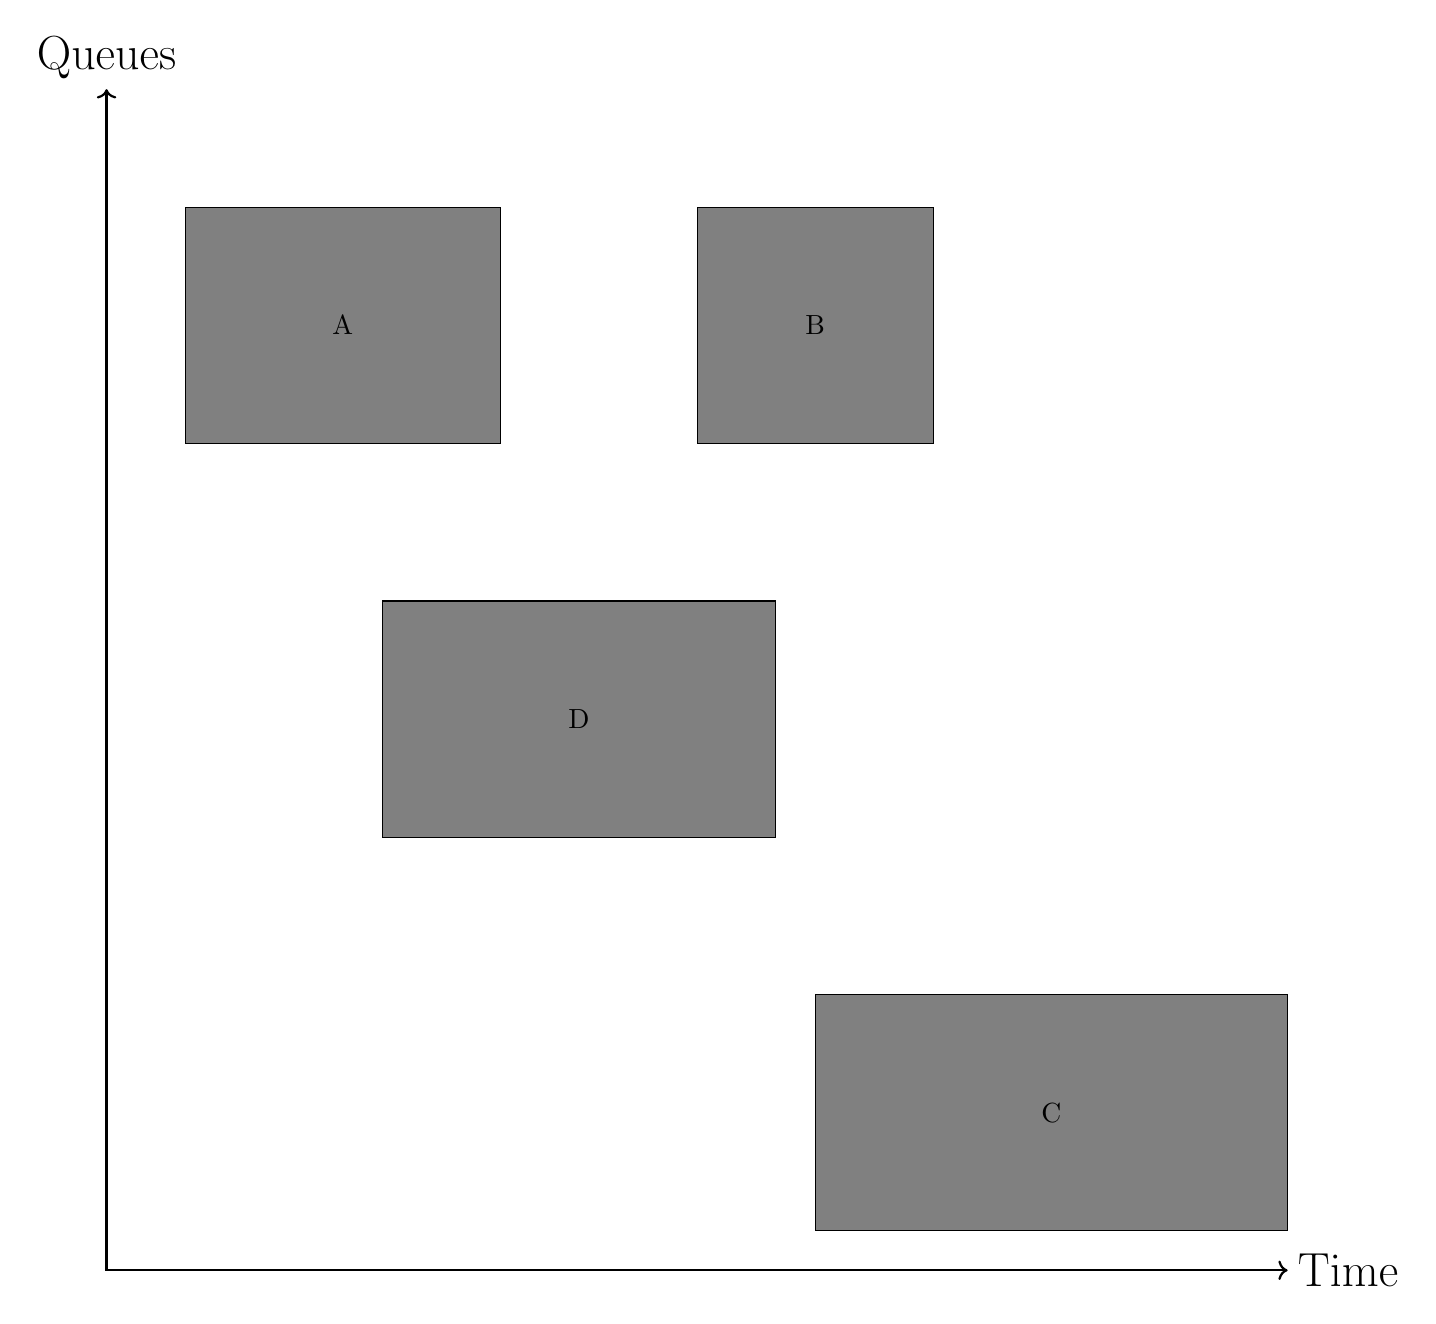
\begin{tikzpicture}
      % Variables
      \def \arrx   {2.0}
      \def \initx  {3.5}
      \def \endx   {8.5}
      \def \depx   {10.0}
      \def \yshift {5}

      % Axis
      \draw [thick,<->] (0,15) node[above]{\LARGE Queues} -- (0,0) -- (15,0) node[right]{\LARGE Time};

      % Rectangles
      \node[rectangle, draw, fill=gray, minimum width=4cm, minimum height = 3cm] at (3,12) {A};
      \node[rectangle, draw, fill=gray, minimum width=3cm, minimum height = 3cm] at (9,12) {B};
      \node[rectangle, draw, fill=gray, minimum width=5cm, minimum height = 3cm] at (6,7) {D};
      \node[rectangle, draw, fill=gray, minimum width=6cm, minimum height = 3cm] at (12,2) {C};

    \end{tikzpicture}
  }
  \label{fig:spacial-and-temporal-constr}
\end{figure}
\end{column}
\end{columns}
\end{frame}

\section{The Position Allocation Problem Approach With Linear Battery Dynamic}
\label{sec:orga9068dc}
\begin{frame}[label={sec:org0a59156}]{Requirements For BEB Implementation}
\begin{columns}
\begin{column}{0.5\columnwidth}
\begin{itemize}
\item Charges must be able to be tracked
\item Service time is unknown
\item Accommodate different charger rates
\item Minimize charger count
\item Minimize consumption cost
\item Encourage slow charger use for battery health
\end{itemize}
\end{column}

\begin{column}{0.5\columnwidth}
\begin{center}
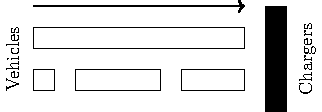
\includegraphics[width=0.8\textwidth]{./img/pap.pdf}
\end{center}

\begin{center}
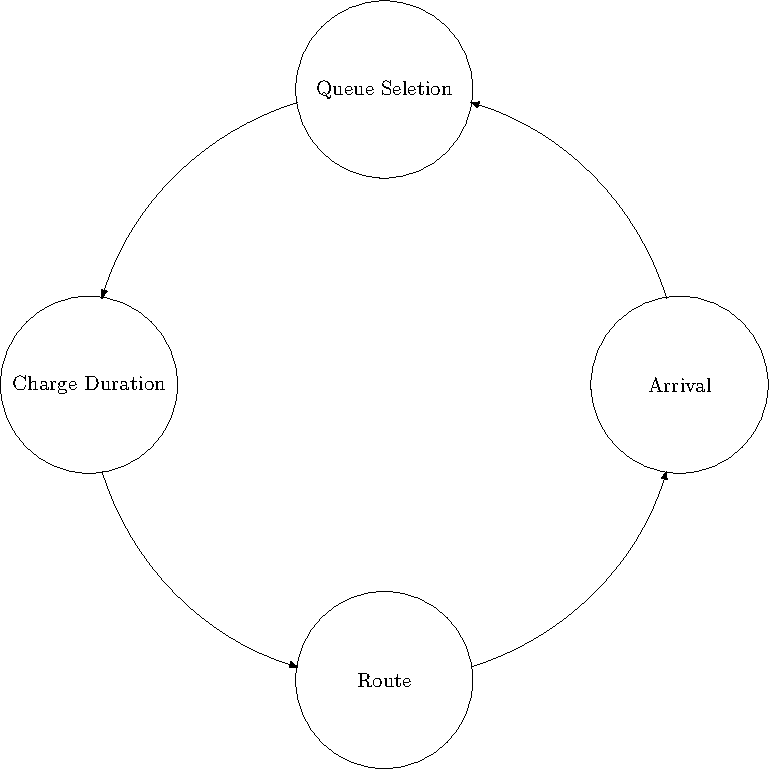
\includegraphics[width=0.7\textwidth]{./img/visit.pdf}
\end{center}
\end{column}
\end{columns}
\end{frame}

\begin{frame}[label={sec:org8090327}]{Mixed Integer Linear Program}
\begin{equation*}
\label{eq:objective}
	\colorboxed{red}{\min \sum_{i=1}^{n_V} \sum_{q=1}^{n_Q} \Big( w_{iq} m_q + g_{iq} \epsilon_q \Big)}
\end{equation*}

\begin{columns}
\begin{column}{0.5\columnwidth}
\begin{beamercolorbox}[shadow=true,rounded=true]{Left}
{\small
\begin{equation*}
\colorboxed{blue}{
\begin{array}{l}
    u_j - u_i - s_i - (\sigma_{ij} - 1)T \geq 0 \\
    v_j - v_i - (\psi_{ij} - 1)n_Q \geq 1 \\
    \sigma_{ij} + \sigma_{ji} \leq 1 \\
    \psi_{ij} + \psi_{ji} \leq 1 \\
    \sigma_{ij} + \sigma_{ji} + \psi_{ij} + \psi_{ji} \geq 1 \\
\end{array}}
\end{equation*}
\begin{equation*}
\colorboxed{orange}{
\begin{array}{l}
    \sum_{q=1}^{n_Q} w_{iq} = 1 \\
    v_i = \sum_{q=1}^{n_Q} qw_{iq} \\
\end{array}}
\end{equation*}
}
\end{beamercolorbox}
\end{column}

\begin{column}{0.5\columnwidth}
{\small
\begin{equation*}
\colorboxed{purple}{
\begin{array}{l}
  s_i + u_i = d_i \\
  a_i \leq u_i \leq (T - s_i) \\
  d_i \leq \tau_i \\
\end{array}}
\end{equation*}
\begin{equation*}
\colorboxed{green}{
\begin{array}{l}
  \eta_i + \sum_{q=1}^{n_Q} g_{iq} r_q - \Delta_i = \eta_{\gamma_i} \\
  \eta_i + \sum_{q=1}^{n_Q} g_{iq} r_q - \Delta_i \geq \nu_{\Gamma_i} \kappa_{\Gamma_i} \\
  \eta_i + \sum_{q=1}^{n_Q} g_{iq} r_q \leq \kappa_{\Gamma_i} \\
  \eta_{\Gamma^0_b} = \alpha_{\Gamma_i} \kappa_{\Gamma_i} \\
  \eta_{\Gamma^f_b} \geq \beta_{\Gamma_b} \kappa_{\Gamma_b}    \\
\end{array}}
\end{equation*}
}
\end{column}
\end{columns}
\end{frame}

\begin{frame}[label={sec:orgce1f86f}]{Queuing Constraints}
\begin{columns}
\begin{column}{0.4\columnwidth}
\begin{equation*}
\colorboxed{blue}{
\begin{array}{l}
    u_j - u_i - s_i - (\sigma_{ij} - 1)T \geq 0 \\
    v_j - v_i - (\psi_{ij} - 1)n_Q \geq 1 \\
    \sigma_{ij} + \sigma_{ji} \leq 1 \\
    \psi_{ij} + \psi_{ji} \leq 1 \\
    \sigma_{ij} + \sigma_{ji} + \psi_{ij} + \psi_{ji} \geq 1 \\
\end{array}}
\end{equation*}

\noindent\rule{\textwidth}{0.5pt}

\begin{itemize}
\item Used to ensure that gray rectangles do not overlap
\item \(\sigma_{ij}\) establishes temporal ordering when active
\item \(\psi_{ij}\) establishes spacial ordering when active
\end{itemize}
\end{column}

\begin{column}{0.6\columnwidth}
\begin{figure}
    \centering
    \scalebox{0.4}{
      \centering
        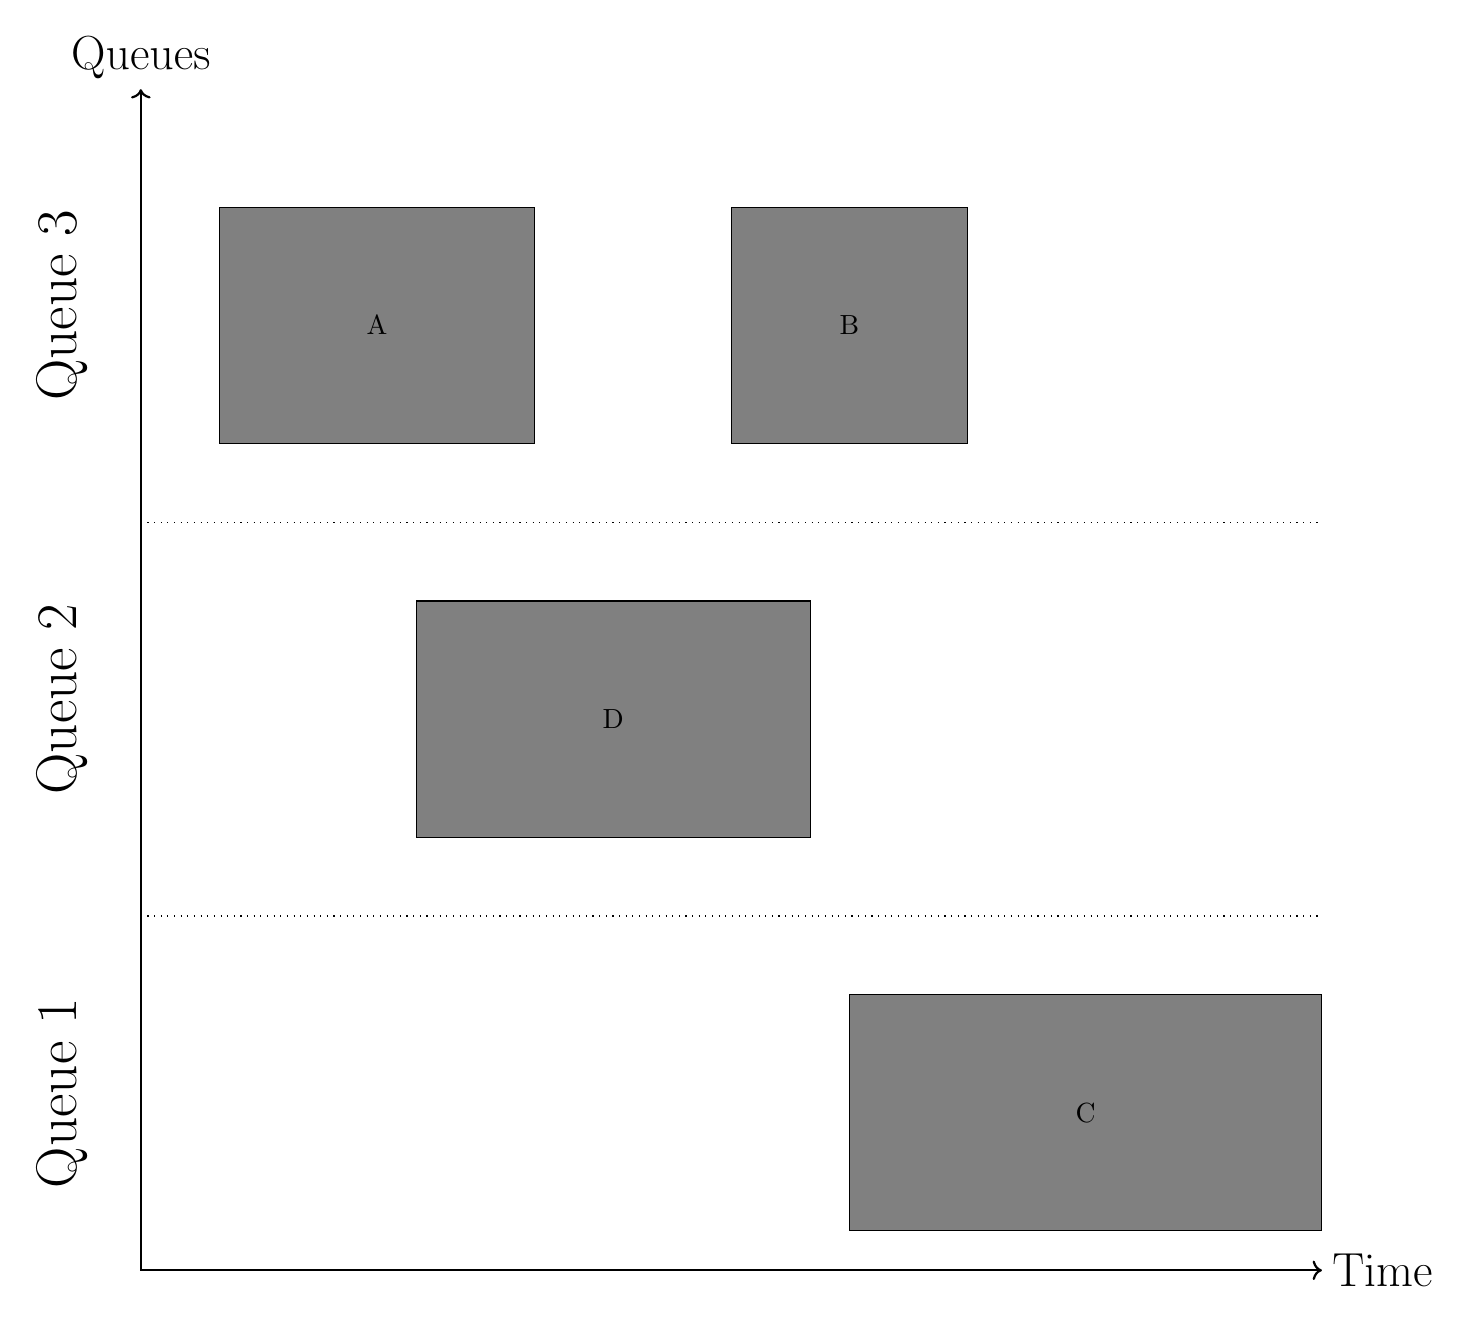
\begin{tikzpicture}
          % Variables
          \def \arrx   {2.0}
          \def \initx  {3.5}
          \def \endx   {8.5}
          \def \depx   {10.0}
          \def \yshift {5}

          % Axis
          \draw [thick,<->] (0,15) node[above]{\LARGE Queues} -- (0,0) -- (15,0) node[right]{\LARGE Time};

          % Rectangles
          \node[rectangle, draw, fill=gray, minimum width=4cm, minimum height = 3cm] at (3,12) {A};
          \node[rectangle, draw, fill=gray, minimum width=3cm, minimum height = 3cm] at (9,12) {B};
          \node[rectangle, draw, fill=gray, minimum width=5cm, minimum height = 3cm] at (6,7) {D};
          \node[rectangle, draw, fill=gray, minimum width=6cm, minimum height = 3cm] at (12,2) {C};

          % Y-axis labels
          \node[rotate=90] at (-1, 2.25) {\huge Queue 1};
          \node[rotate=90] at (-1, 7.25) {\huge Queue 2};
          \node[rotate=90] at (-1, 12.25) {\huge Queue 3};

          % Horizontal lines
          \draw[dotted] (0, 4.5) -- (15, 4.5);
          \draw[dotted] (0, 9.5) -- (15, 9.5);

        \end{tikzpicture}
      }
      \label{fig:spacial-and-temporal-constr}
\end{figure}
\end{column}
\end{columns}
\end{frame}

\begin{frame}[label={sec:org840fd15}]{Parameters}
\begin{columns}
\begin{column}{0.3\columnwidth}
\begin{center}
\begin{tabular}{l|l}
\hline
Parameter & Value\\[0pt]
\hline
Execution & 2 hr\\[0pt]
\(T\) & 24 hr\\[0pt]
\(n_V\) & 338\\[0pt]
\(n_A\) & 35\\[0pt]
\(\alpha_i\) & 90\%\\[0pt]
\(\nu_i\) & 25\%\\[0pt]
\(\beta_i\) & 70\%\\[0pt]
\(m_q\) & 1000q\\[0pt]
\hline
\end{tabular}
\end{center}
\end{column}

\begin{column}{0.7\columnwidth}
\begin{figure}
    \centering
    \scalebox{0.4}{
      \centering
        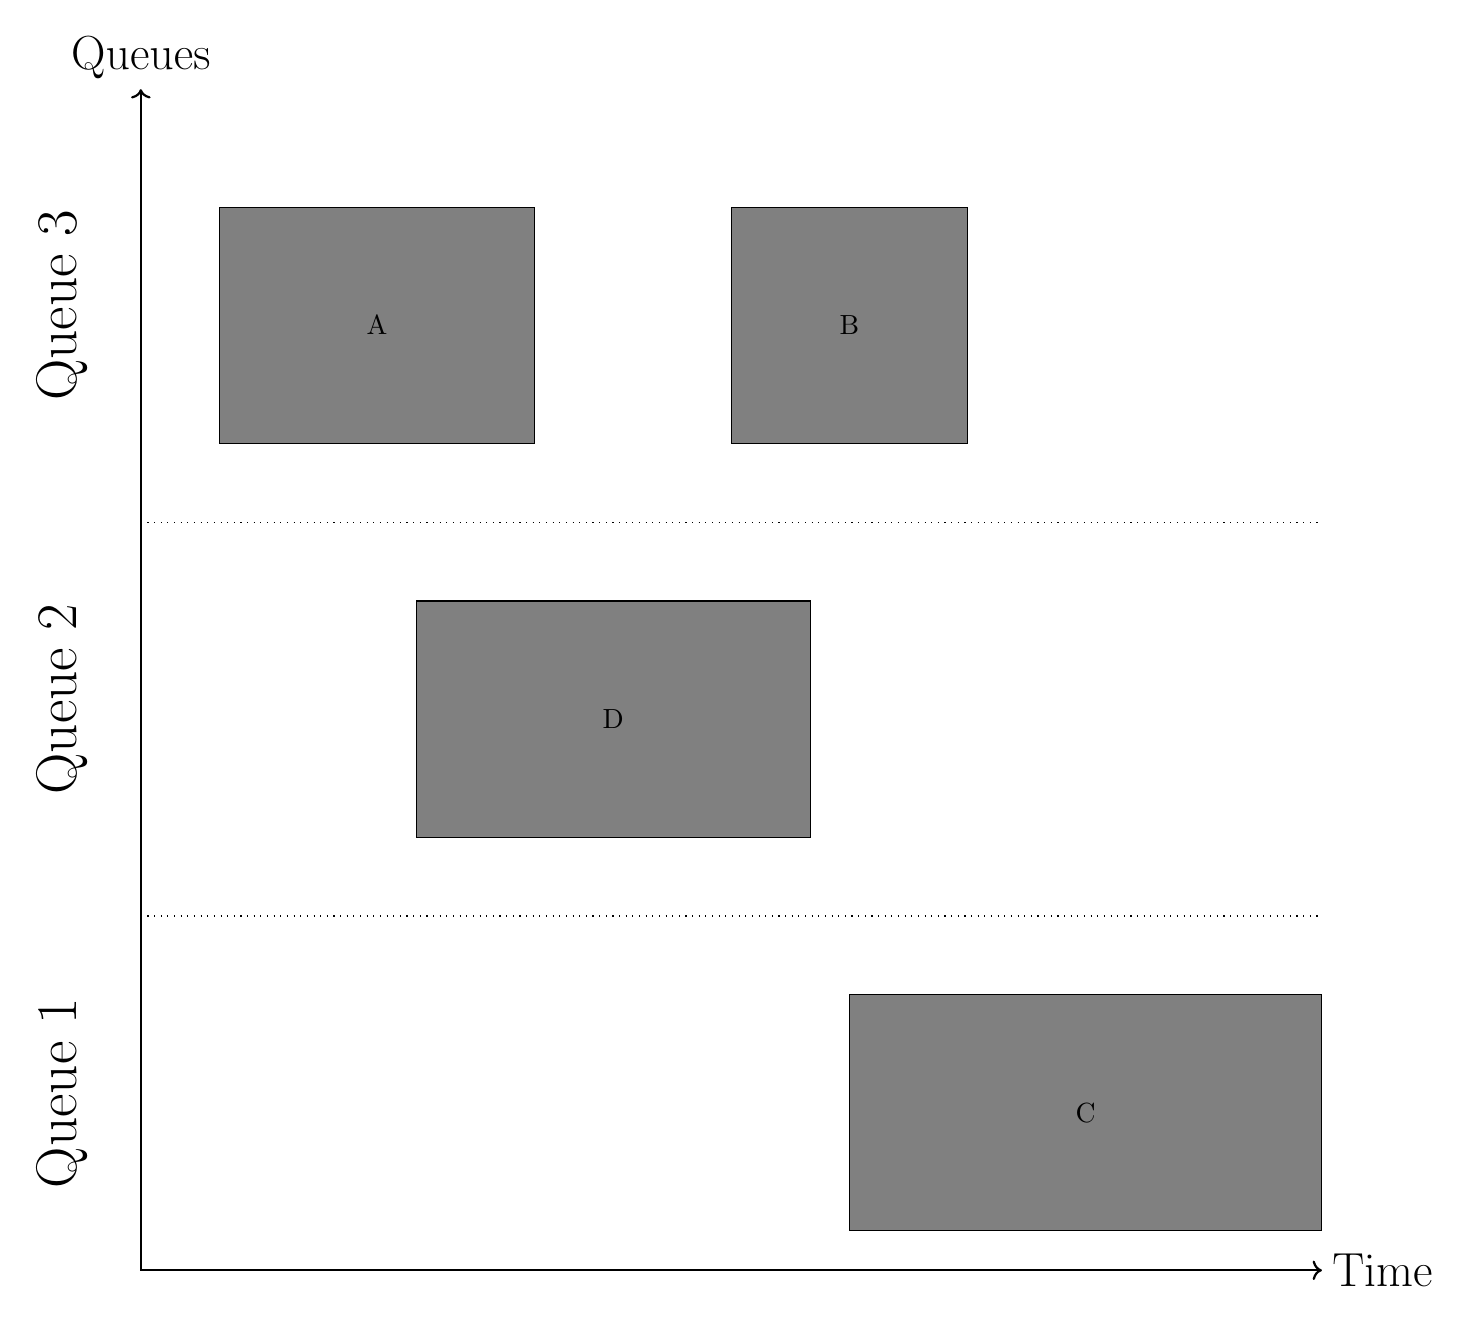
\begin{tikzpicture}
          % Variables
          \def \arrx   {2.0}
          \def \initx  {3.5}
          \def \endx   {8.5}
          \def \depx   {10.0}
          \def \yshift {5}

          % Axis
          \draw [thick,<->] (0,15) node[above]{\LARGE Queues} -- (0,0) -- (15,0) node[right]{\LARGE Time};

          % Rectangles
          \node[rectangle, draw, fill=gray, minimum width=4cm, minimum height = 3cm] at (3,12) {A};
          \node[rectangle, draw, fill=gray, minimum width=3cm, minimum height = 3cm] at (9,12) {B};
          \node[rectangle, draw, fill=gray, minimum width=5cm, minimum height = 3cm] at (6,7) {D};
          \node[rectangle, draw, fill=gray, minimum width=6cm, minimum height = 3cm] at (12,2) {C};

          % Y-axis labels
          \node[rotate=90] at (-1, 2.25) {\huge Queue 1};
          \node[rotate=90] at (-1, 7.25) {\huge Queue 2};
          \node[rotate=90] at (-1, 12.25) {\huge Queue 3};

          \draw[dotted] (0, 4.5) -- (15, 4.5);
          \draw[dotted] (0, 9.5) -- (15, 9.5);

        \end{tikzpicture}
      }
      \label{fig:spacial-and-temporal-constr}
\end{figure}
\end{column}
\end{columns}
\end{frame}

\begin{frame}[label={sec:orgc48fe99}]{Schedules}
\begin{columns}
\begin{column}{0.5\columnwidth}
\begin{figure}[htpb]
\centering
    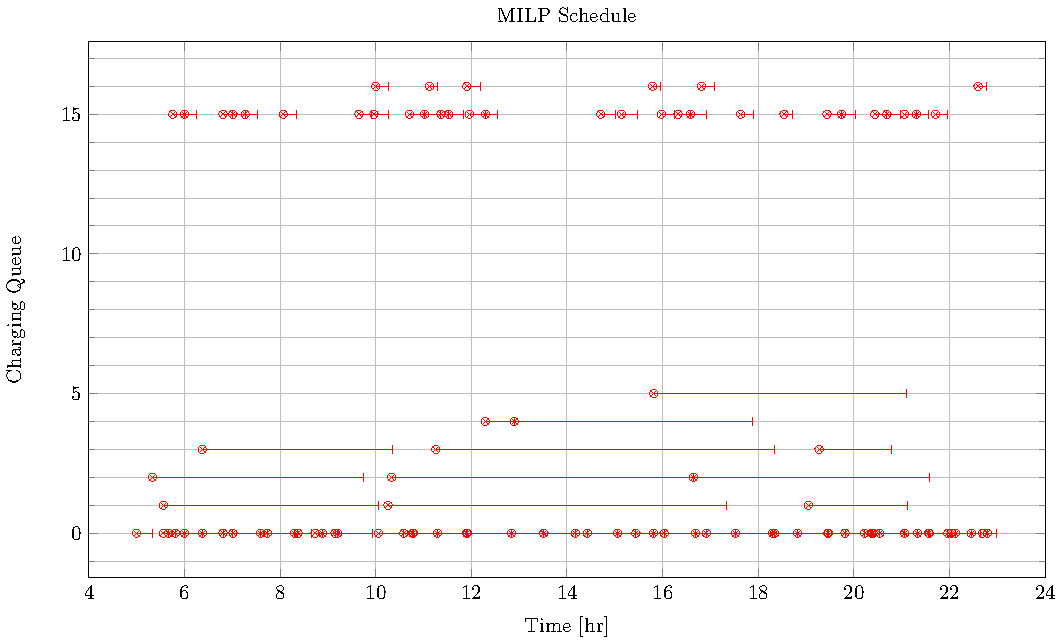
\includegraphics[width=\textwidth]{img/milp-pap/schedule-milp-pap}
\end{figure}

\begin{itemize}
\item Slow chargers utilized more frequently
\item Fast chargers utilized sparingly
\end{itemize}
\end{column}

\begin{column}{0.5\columnwidth}
\begin{figure}[htpb]
\centering
    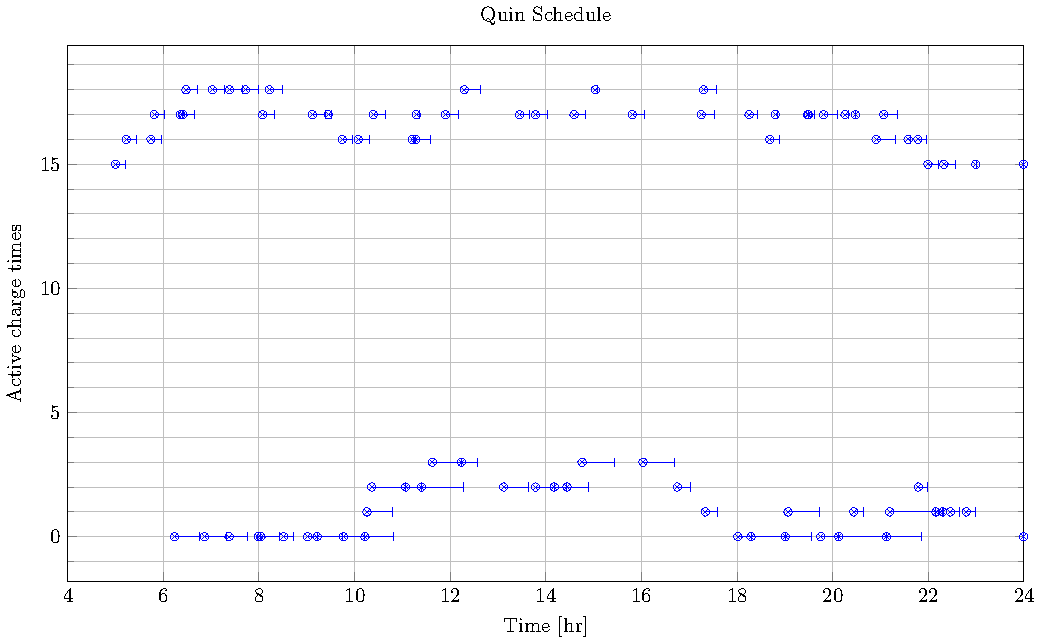
\includegraphics[width=\textwidth]{img/milp-pap/schedule-qin}
\end{figure}

\begin{itemize}
\item Slow chargers used for short durations
\item Extensive use of fast chargers
\end{itemize}
\end{column}
\end{columns}
\end{frame}

\begin{frame}[label={sec:org4fa67c8}]{SOC And Energy Use}
\begin{columns}
\begin{column}{0.5\columnwidth}
\begin{center}
\begin{tabular}{l|cccc}
\hline
 & MILP [kWh] & Qin [kWh]\\[0pt]
\hline
Mean & 265.873 & 355.93\\[0pt]
Min & 97.04 & 0.000\\[0pt]
Max & 388 & 368.354\\[0pt]
\hline
\end{tabular}
\end{center}

\begin{itemize}
\item SOC of Qin allowed to drop to 0
\item PAP maintained minimum SOC and final SOC
\end{itemize}
\end{column}

\begin{column}{0.5\columnwidth}
\begin{center}
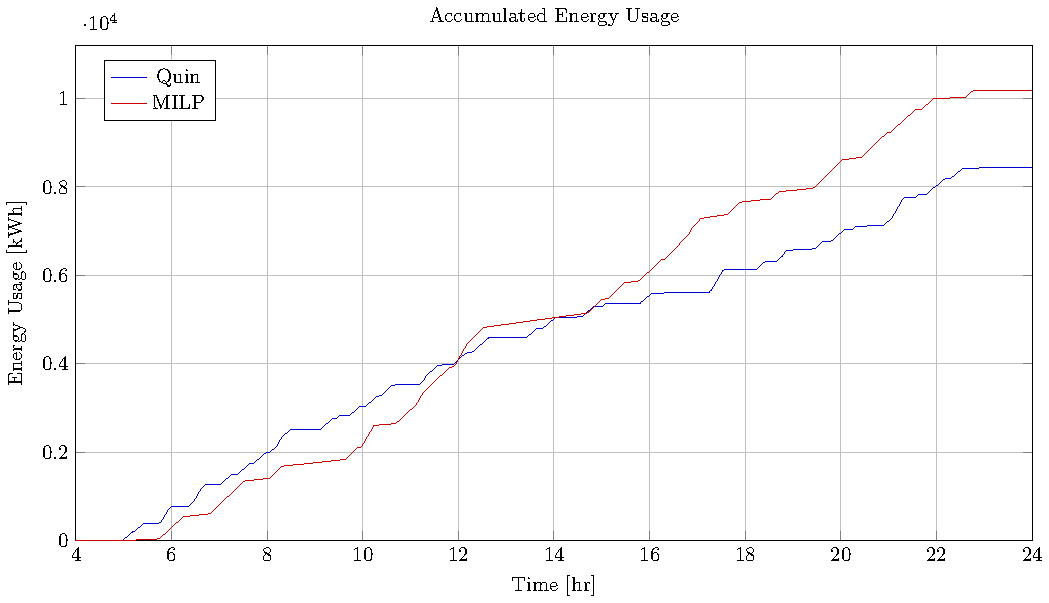
\includegraphics[width=\textwidth]{./img/milp-pap/energy-milp-pap.pdf}
\end{center}

\begin{itemize}
\item PAP accumulated energy is larger due to minimum SOC constraints
\end{itemize}
\end{column}
\end{columns}
\end{frame}

\section{The Simulated Annealing Approach With Linear Battery Dynamics}
\label{sec:orgabc6205}
\begin{frame}[label={sec:org09dc60b}]{Objective Function And Constraints}
\begin{equation*}
  \colorboxed{red}{J(\mathbb{I}) = z_d p_d + \sum_{i=1}^{n_V} \Big[ \epsilon_{q_i}r_{q_i} + z_p \phi_i(\eta_i - \nu_{b_i} \kappa_{b_i}) + z_c r_{q_i} s_i \Big]}
\end{equation*}

\begin{columns}
\begin{column}{0.5\columnwidth}
{\footnotesize
\begin{itemize}
\item \(p_d\): Demand cost
\begin{itemize}
\item \(p_{T_p,h} = \frac{1}{T_p} \sum_{k = h-\frac{T_p}{dt}+1}^h p_k\; dt\)
\item \(p_{max} = \max\limits_{k \in [h-\frac{T_p}{dt}+1, h]}\; p_{T_p,h}\)
\item \(p_d = \max(p_{fix}, p_{max})\)
\end{itemize}

\begin{equation*}
  \colorboxed{purple}{
      \begin{array}{c}
        s_i = d_i - u_i \\
        a_i \leq u_i \leq d_i \le e_i \le \mathcal{T} \\
  \end{array}}
\end{equation*}

\begin{equation*}
  \colorboxed{green}{
      \begin{array}{c}
        \eta_{\xi_i} = \eta_{i} + r_{q_i}s_i - \Delta_i \\
        \kappa_{b_i} \geq \eta_{i} + r_{q_i}s_i \\
  \end{array}}
\end{equation*}
\end{itemize}
}
\end{column}

\begin{column}{0.5\columnwidth}
{\footnotesize
\begin{itemize}
\item \(\epsilon_{q_i}r_{q_i}\): Assignment Cost
\item \(z_p \phi_i(\eta_i - \nu_{b_i} \kappa_{b_i})\): Penalty Function
\item \(z_c r_{q_i} s_i\): Consumption Cost

\begin{equation*}
  \colorboxed{blue}{
  \begin{array}{l}
    u_j - d_i - (\sigma_{ij} - 1)T \ge 0 \\
    q_j - q_i - 1 - (\psi_{ij} - 1)Q \ge 0 \\
    \sigma_{ij} + \sigma_{ji} \le 1 \\
    \psi_{ij} + \psi_{ji} \le 1 \\
    \sigma_{ij} + \sigma_{ji} + \psi_{ij} + \psi_{ji} \ge 1
  \end{array}}
\end{equation*}
\end{itemize}
}
\end{column}
\end{columns}
\end{frame}

\begin{frame}[label={sec:org9346e1e}]{Parameters}
\begin{columns}
\begin{column}{0.5\columnwidth}
{\small
\alert{NOTES}:
\begin{itemize}
\item Results are different from what is presented in the thesis
\item BPAP model does not take demand cost into consideration
\end{itemize}
}

\begin{center}
\begin{tabular}{l|c}
\alert{Model} & \alert{Execution Time} [s]\\[0pt]
\hline
BPAP & 1900\\[0pt]
Quick & 1533\\[0pt]
Heuristic & 1916\\[0pt]
\hline
\end{tabular}
\end{center}

\begin{columns}
\begin{column}{0.5\columnwidth}
\begin{itemize}
\item \(T_0 = 90000\)
\item \(\beta = 0.997\)
\end{itemize}
\end{column}

\begin{column}{0.5\columnwidth}
\begin{itemize}
\item \(|t| = 3797\)
\item \(n_K = 500\)
\end{itemize}
\end{column}
\end{columns}
\end{column}

\begin{column}{0.5\columnwidth}
\begin{figure}
    \centering
    \scalebox{0.4}{
      \centering
        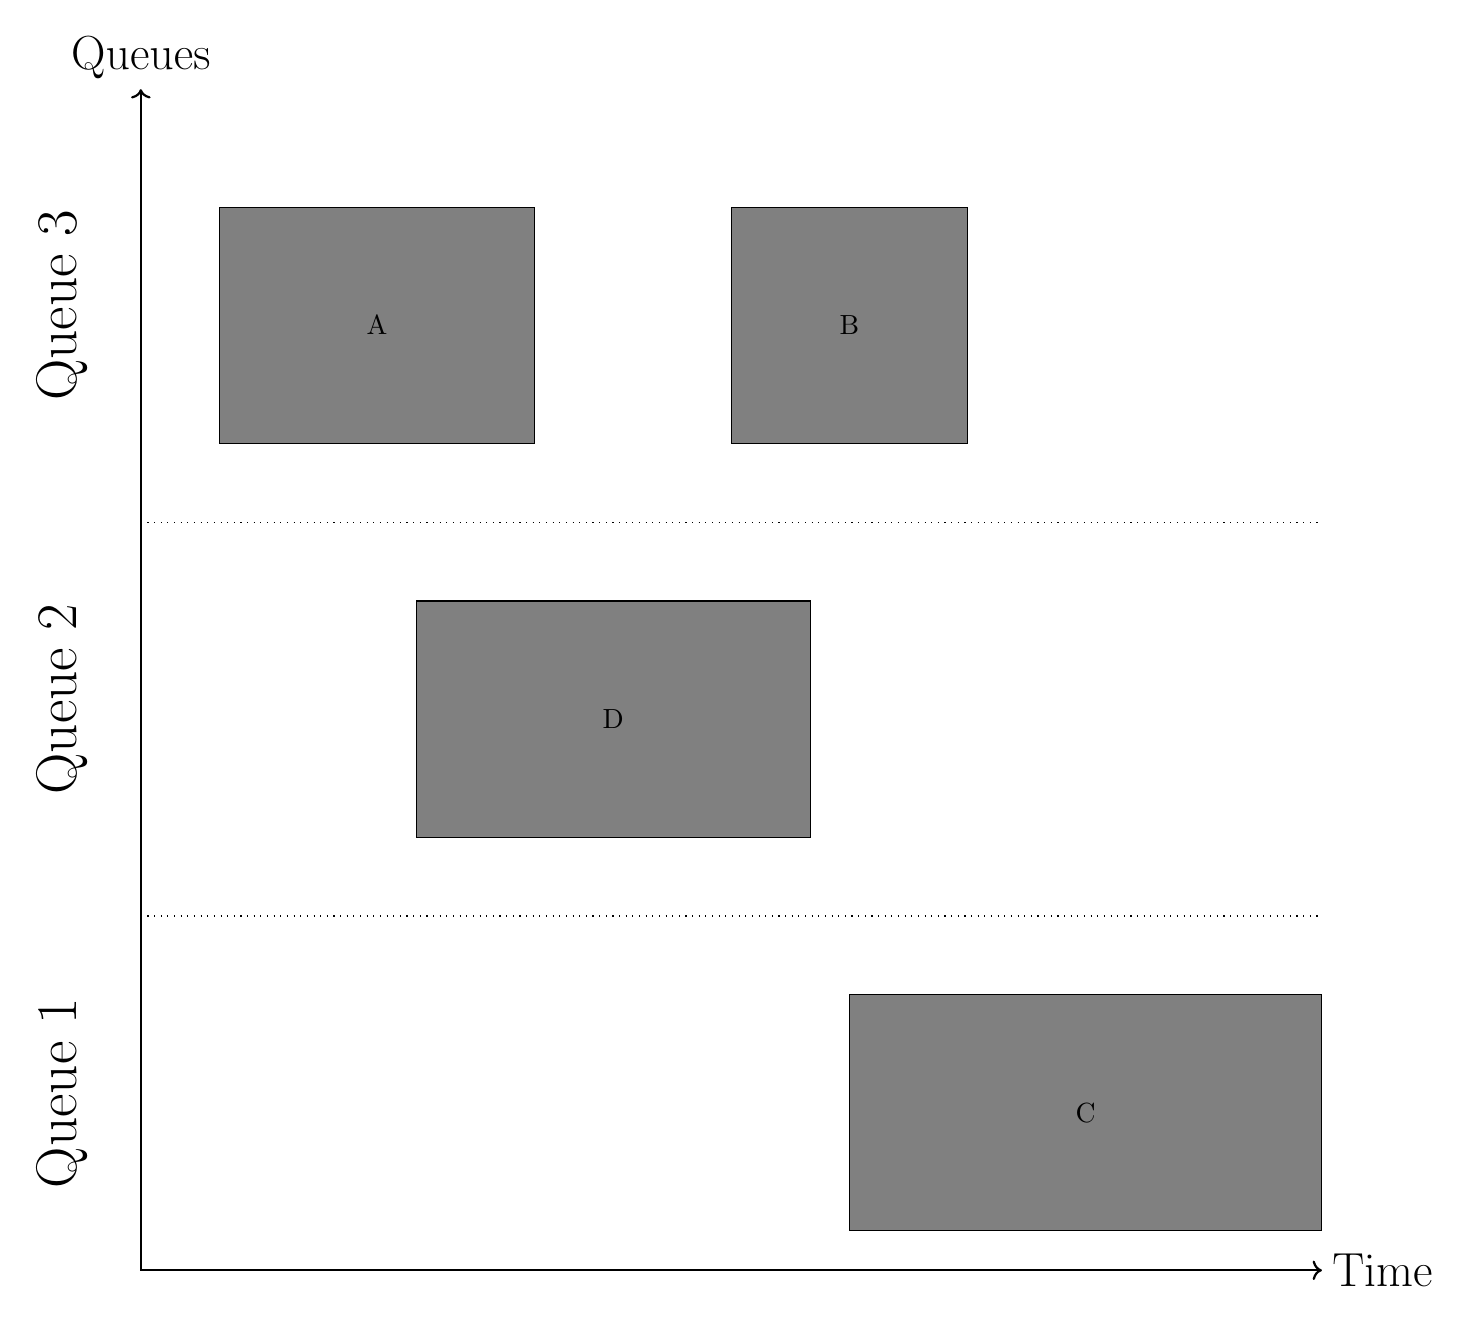
\begin{tikzpicture}
          % Variables
          \def \arrx   {2.0}
          \def \initx  {3.5}
          \def \endx   {8.5}
          \def \depx   {10.0}
          \def \yshift {5}

          % Axis
          \draw [thick,<->] (0,15) node[above]{\LARGE Queues} -- (0,0) -- (15,0) node[right]{\LARGE Time};

          % Rectangles
          \node[rectangle, draw, fill=gray, minimum width=4cm, minimum height = 3cm] at (3,12) {A};
          \node[rectangle, draw, fill=gray, minimum width=3cm, minimum height = 3cm] at (9,12) {B};
          \node[rectangle, draw, fill=gray, minimum width=5cm, minimum height = 3cm] at (6,7) {D};
          \node[rectangle, draw, fill=gray, minimum width=6cm, minimum height = 3cm] at (12,2) {C};

          % Y-axis labels
          \node[rotate=90] at (-1, 2.25) {\huge Queue 1};
          \node[rotate=90] at (-1, 7.25) {\huge Queue 2};
          \node[rotate=90] at (-1, 12.25) {\huge Queue 3};

          \draw[dotted] (0, 4.5) -- (15, 4.5);
          \draw[dotted] (0, 9.5) -- (15, 9.5);

        \end{tikzpicture}
      }
      \label{fig:spacial-and-temporal-constr}
\end{figure}
\end{column}
\end{columns}
\end{frame}

\begin{frame}[label={sec:org38219b5}]{Schedule}
\begin{columns}
\begin{column}{0.5\columnwidth}
{\scriptsize
\begin{itemize}
\item Qin heavily utilizes fast charger
\item BPAP emphasizes slow queues, but utilizes fast chargers readily
\end{itemize}
}

\begin{figure}
\begin{subfigure}[t]{\textwidth}
\centering
    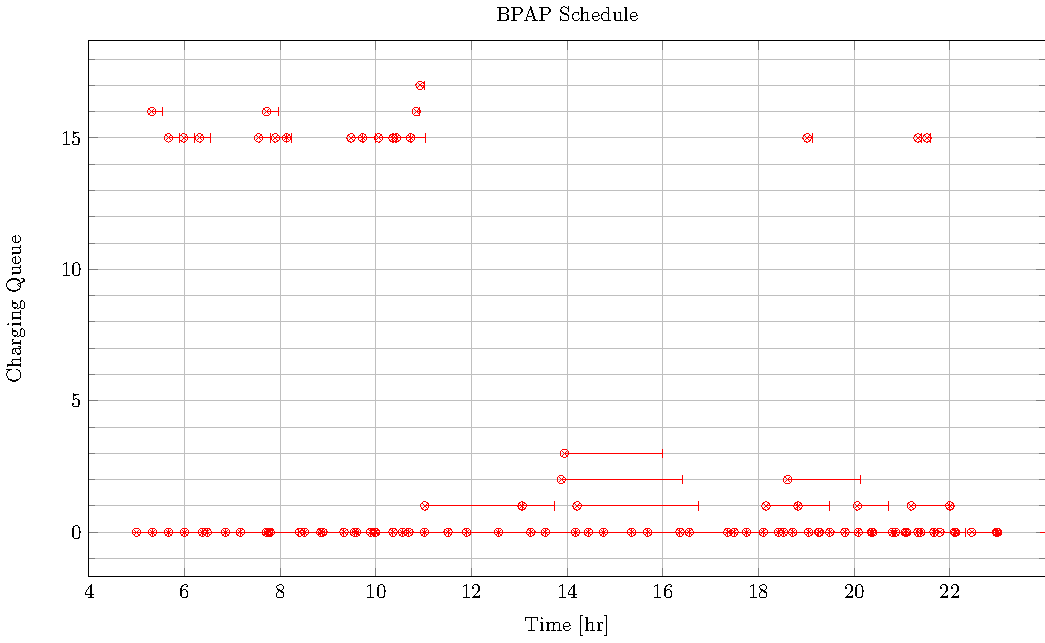
\includegraphics[width=0.7\textwidth]{img/sa-pap-paper-good/schedule-milp}
\end{subfigure}
\begin{subfigure}[t]{\textwidth}
\centering
    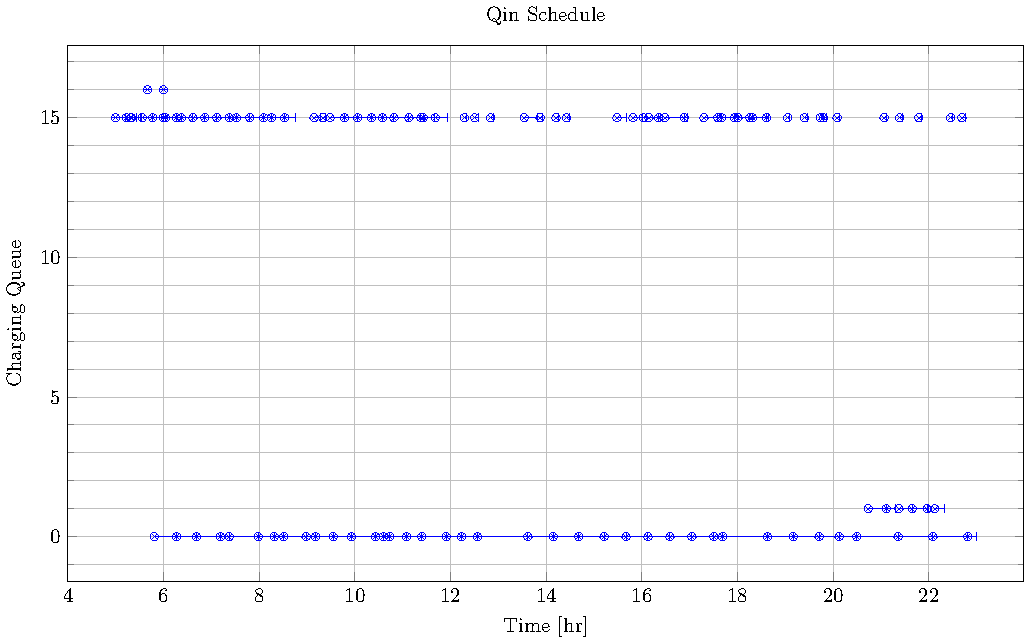
\includegraphics[width=0.7\textwidth]{img/sa-pap-paper-good/schedule-qin}
\end{subfigure}
\end{figure}
\end{column}

\begin{column}{0.5\columnwidth}
{\scriptsize
\begin{itemize}
\item SA techniques heavily utilize slow charging
\item SA techniques utilize fast chargers more sparingly
\end{itemize}
}

\begin{figure}
\begin{subfigure}[t]{\textwidth}
\centering
    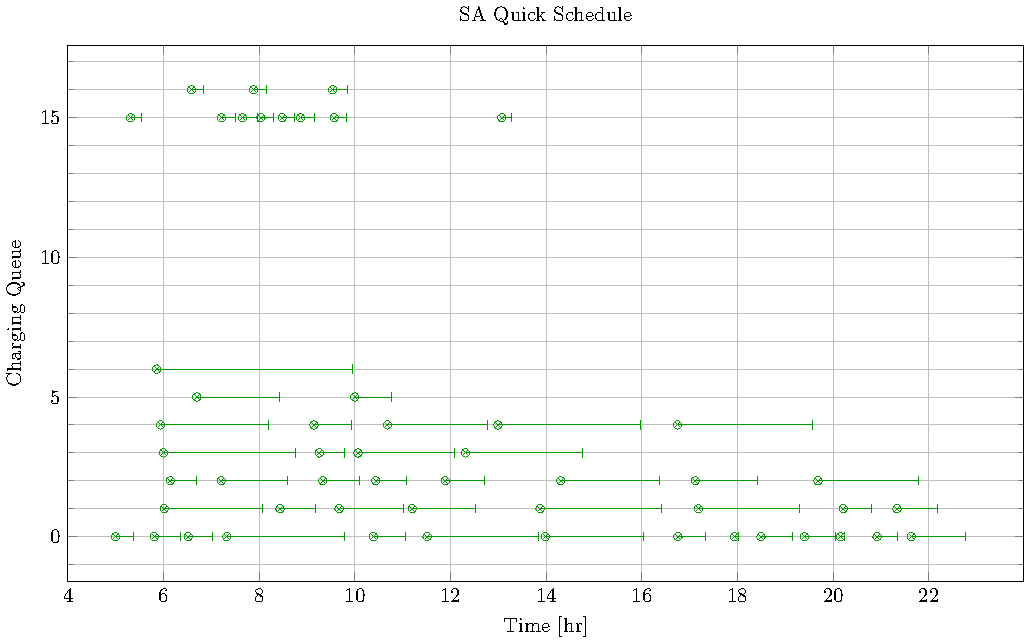
\includegraphics[width=0.7\textwidth]{img/sa-pap-paper-good/schedule-sa-quick}
\end{subfigure}
\begin{subfigure}[t]{\textwidth}
\centering
    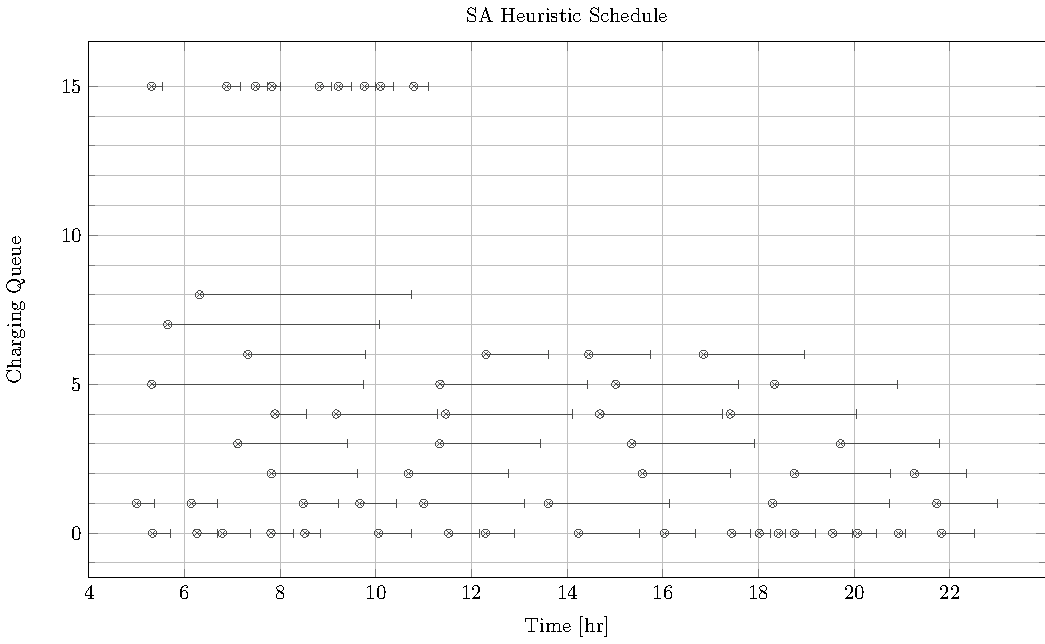
\includegraphics[width=0.7\textwidth]{img/sa-pap-paper-good/schedule-sa-heuristic}
\end{subfigure}
\end{figure}
\end{column}
\end{columns}
\end{frame}

\begin{frame}[label={sec:org3322cc5}]{Power}
\begin{columns}
\begin{column}{0.5\columnwidth}
\begin{figure}[htpb]
\centering
    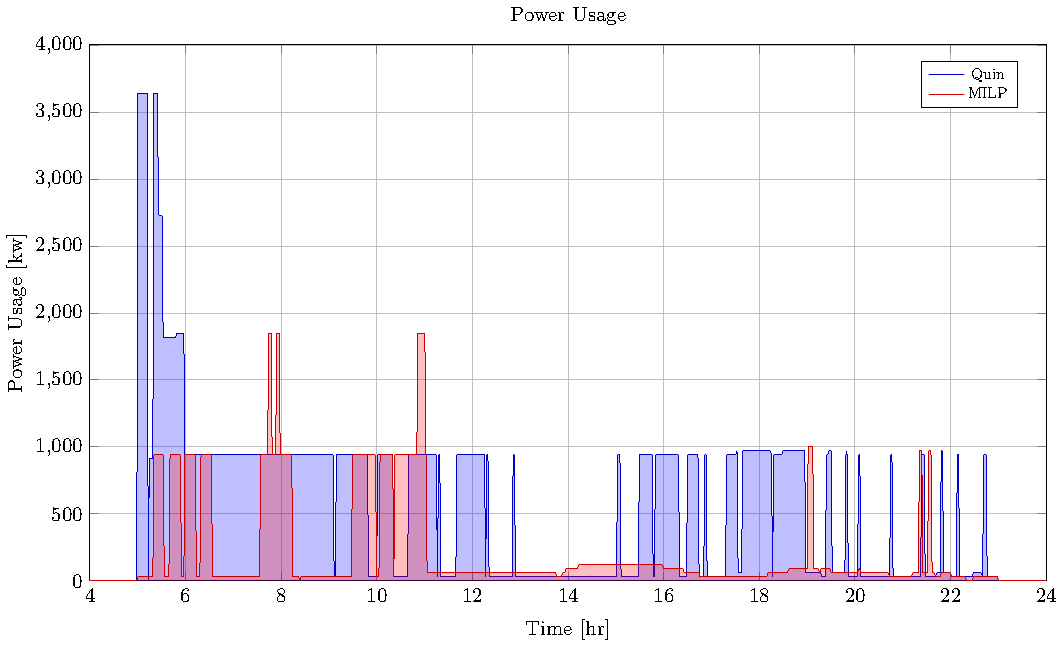
\includegraphics[width=\textwidth]{img/sa-pap-paper-good/power-milp-qin}
\end{figure}

\begin{itemize}
\item Heuristic SA maintained the lowest demand peak
\end{itemize}
\end{column}

\begin{column}{0.5\columnwidth}
\begin{figure}[htpb]
\centering
    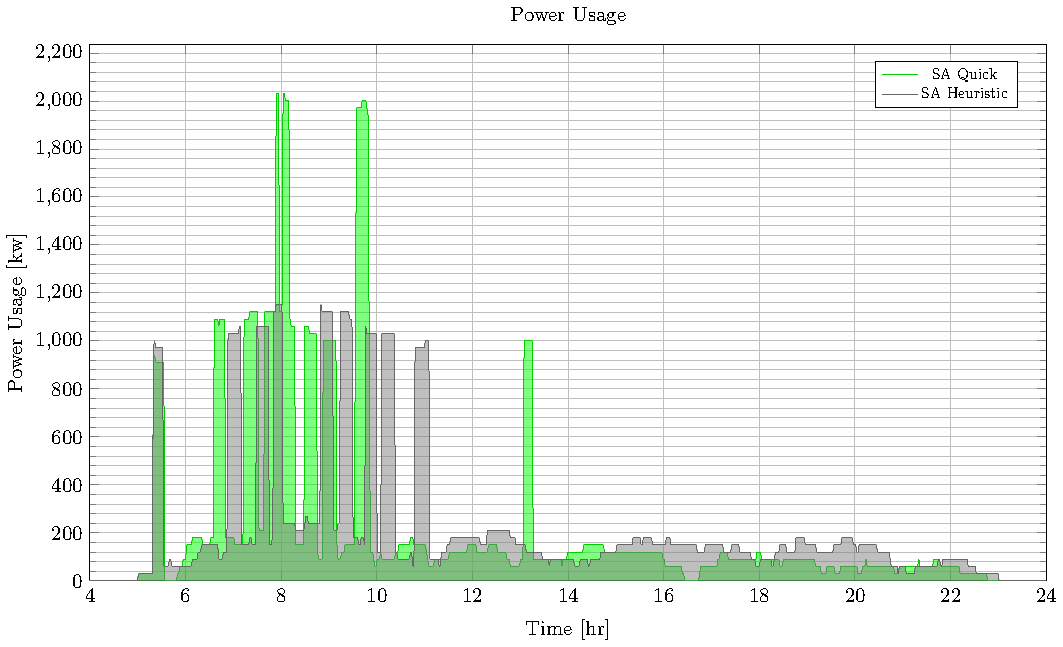
\includegraphics[width=\textwidth]{img/sa-pap-paper-good/power-sa}
\end{figure}


\begin{itemize}
\item Quick SA peak demand comparable to the PAP peak
\end{itemize}
\end{column}
\end{columns}
\end{frame}

\begin{frame}[label={sec:org5e624d9}]{SOC and Energy}
\begin{columns}
\begin{column}{0.3\columnwidth}
\begin{itemize}
\item SOC threshold deficits:
\begin{itemize}
\item quick: 2.24 kWh
\item heuristic: 5.74 kWh
\end{itemize}
\item Energy delta:
\begin{itemize}
\item quick: 191.47 kWh
\item heuristic: 58.46 kWh
\end{itemize}
\item Trade off of the lower peak demand
\end{itemize}
\end{column}

\begin{column}{0.7\columnwidth}
\begin{figure}[htpb]
\centering
    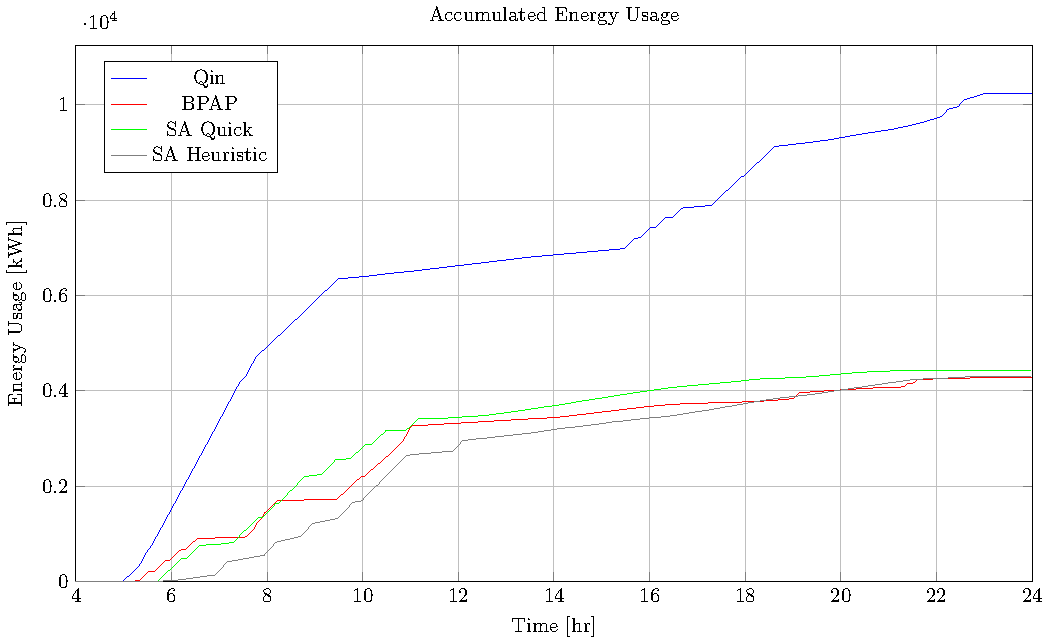
\includegraphics[width=\textwidth]{img/sa-pap-paper-good/energy}
\end{figure}
\end{column}
\end{columns}
\end{frame}

\begin{frame}[label={sec:org189bc8b}]{Scores and Energy}
\begin{columns}
\begin{column}{0.35\columnwidth}
\begin{center}
\begin{tabular}{l|c}
\hline
Schedule & Score\\[0pt]
\hline
BPAP & \num{18500000}\\[0pt]
Qin-Modified & \num{34578526}\\[0pt]
Heuristic & \num{11673937}\\[0pt]
Quick & \num{11234577}\\[0pt]
\hline
\end{tabular}
\end{center}
\end{column}

\begin{column}{0.75\columnwidth}
\begin{figure}[htpb]
\centering
    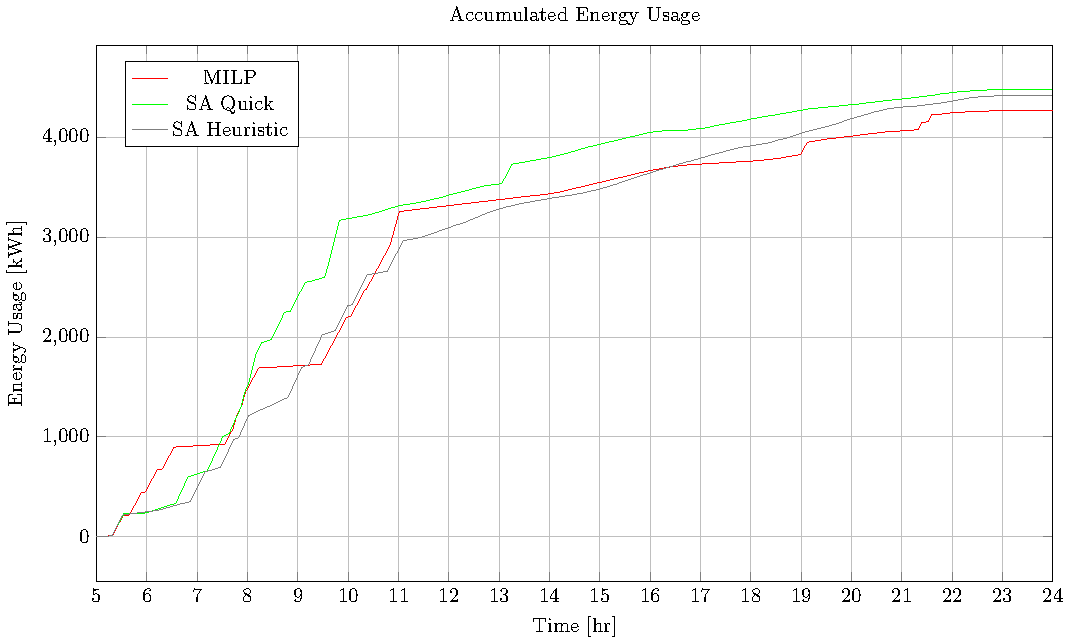
\includegraphics[width=0.9\textwidth]{img/sa-pap-paper-good/energy-zoom}
\end{figure}
\end{column}
\end{columns}
\end{frame}

\section{Summary and Questions}
\label{sec:org78d6f15}
\begin{frame}[label={sec:org2a36cf0}]{Summary}
\end{frame}
\begin{frame}[label={sec:org96d2638}]{Publications}
\end{frame}
\begin{frame}[label={sec:orgbd28e47}]{}
\centering
\Huge Questions?
\end{frame}

\appendix
\begin{frame}[label={sec:orgd34364b}]{}
\centering
\Huge Appendix
\end{frame}

\begin{frame}[label={sec:org0c3b817}]{}
\centering
\Huge SA with Non-Linear Battery Dynamics
\end{frame}

\begin{frame}[label={sec:org31e54cb}]{Introduction}
\begin{columns}
\begin{column}{0.3\columnwidth}
\begin{itemize}
\item Higher fidelity in approximating charge at high SOC
\item Implemented in SA for simplicity
\end{itemize}
\end{column}

\begin{column}{0.7\columnwidth}
\begin{center}
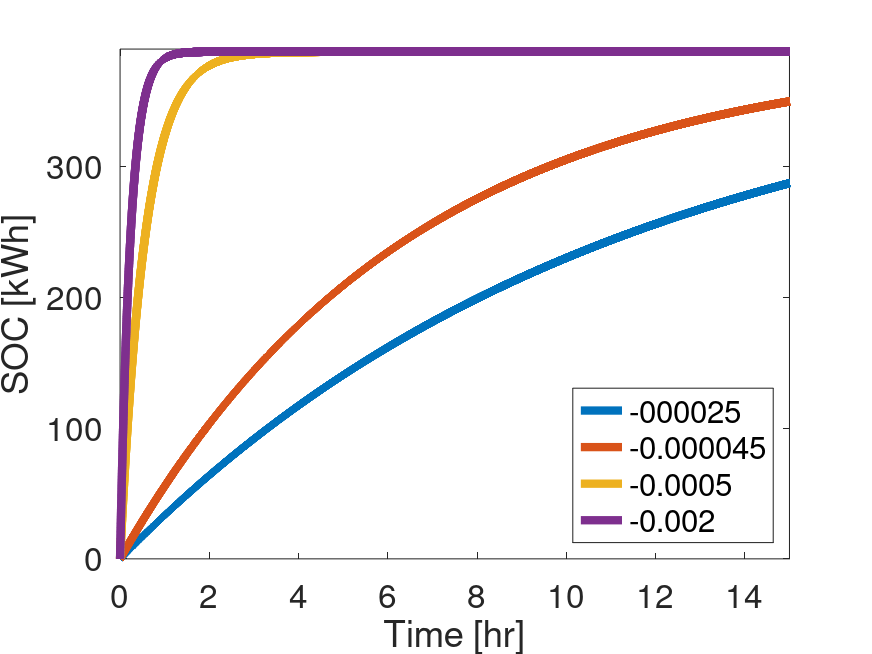
\includegraphics[width=.9\linewidth]{./img/nonlinear-bat.png}
\end{center}
\end{column}
\end{columns}
\end{frame}

\begin{frame}[label={sec:org2a83658}]{Non-Linear Battery Dynamics Model}
\begin{columns}
\begin{column}{0.3\columnwidth}
\begin{equation*}
\eta_{\xi_i} = \bar{a}_q \eta_i - \bar{b}_q \kappa_{b_i}
\end{equation*}

\begin{equation*}
\begin{array}{cc}
  \bar{a}_q = e^{a_q dt} & \bar{b}_q = e^{a_q dt} - 1
\end{array}
\end{equation*}
\end{column}

\begin{column}{0.7\columnwidth}
\begin{center}
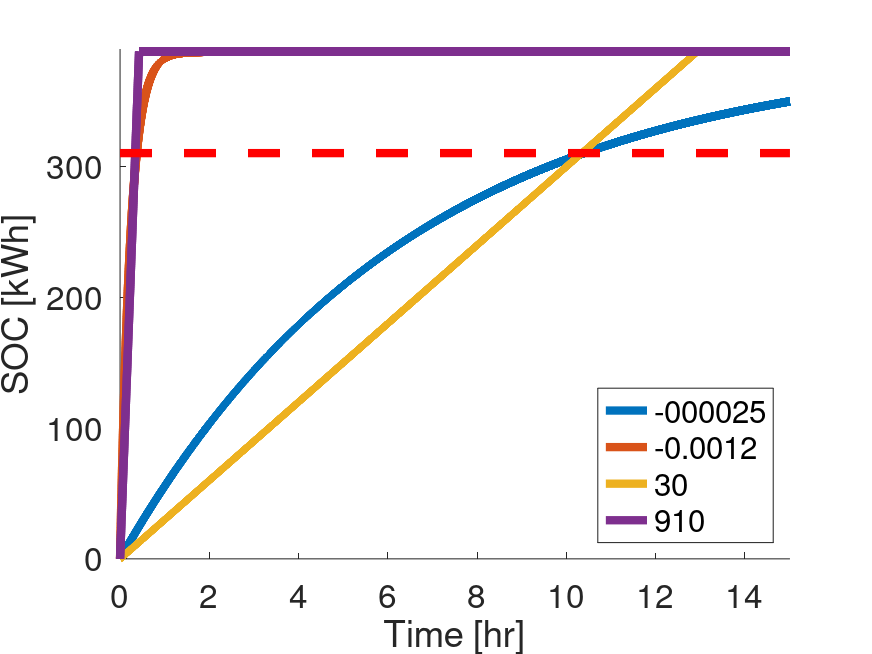
\includegraphics[width=.9\linewidth]{./img/nonlinear-bat-lin.png}
\end{center}
\end{column}
\end{columns}
\end{frame}

\begin{frame}[label={sec:orgfae9996}]{Results}
\begin{columns}
\begin{column}{0.5\columnwidth}
{\scriptsize
\begin{itemize}
\item Minimized demand power
\item Larger energy consumption due to fast charger duration
\end{itemize}
}

\begin{figure}
\begin{subfigure}[t]{\textwidth}
\centering
    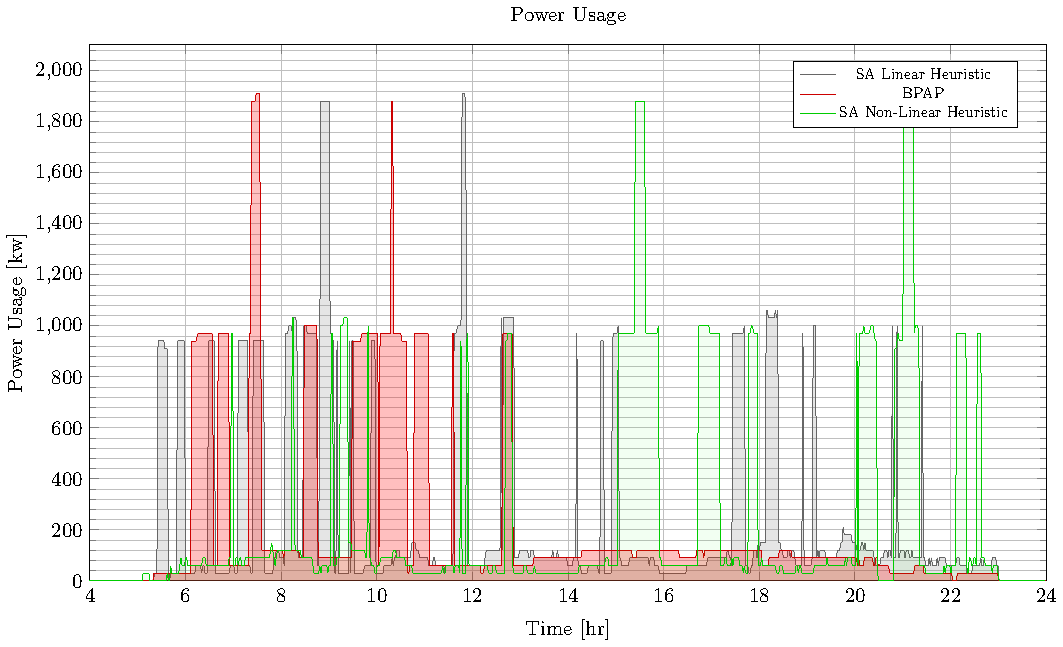
\includegraphics[width=0.7\textwidth]{img/sa-nonlinear/power-sa-nonlinear}
\end{subfigure}
\begin{subfigure}[t]{\textwidth}
\centering
    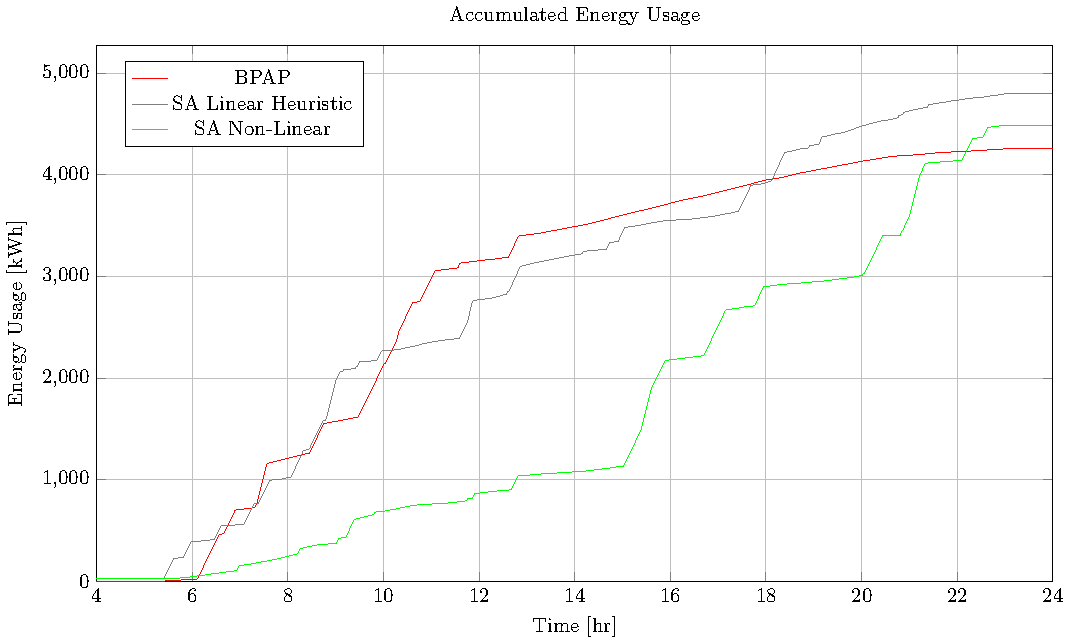
\includegraphics[width=0.7\textwidth]{img/sa-nonlinear/energy-sa-nonlinear}
\end{subfigure}
\end{figure}
\end{column}

\begin{column}{0.5\columnwidth}
{\scriptsize
\begin{itemize}
\item Similar schedule output, longer fast charger durations due to nonlinear model
\item Minimum SOC of 85 kWh
\end{itemize}
}

\begin{figure}
\begin{subfigure}[t]{\textwidth}
\centering
    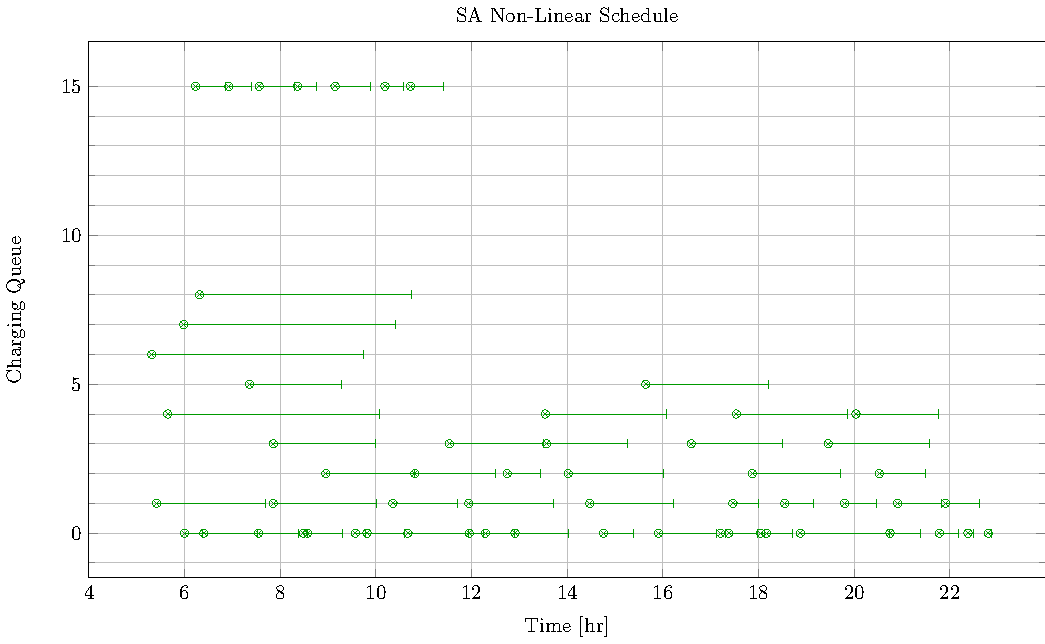
\includegraphics[width=0.7\textwidth]{img/sa-nonlinear/schedule-sa-nonlinear}
\end{subfigure}
\begin{subfigure}[t]{\textwidth}
\centering
    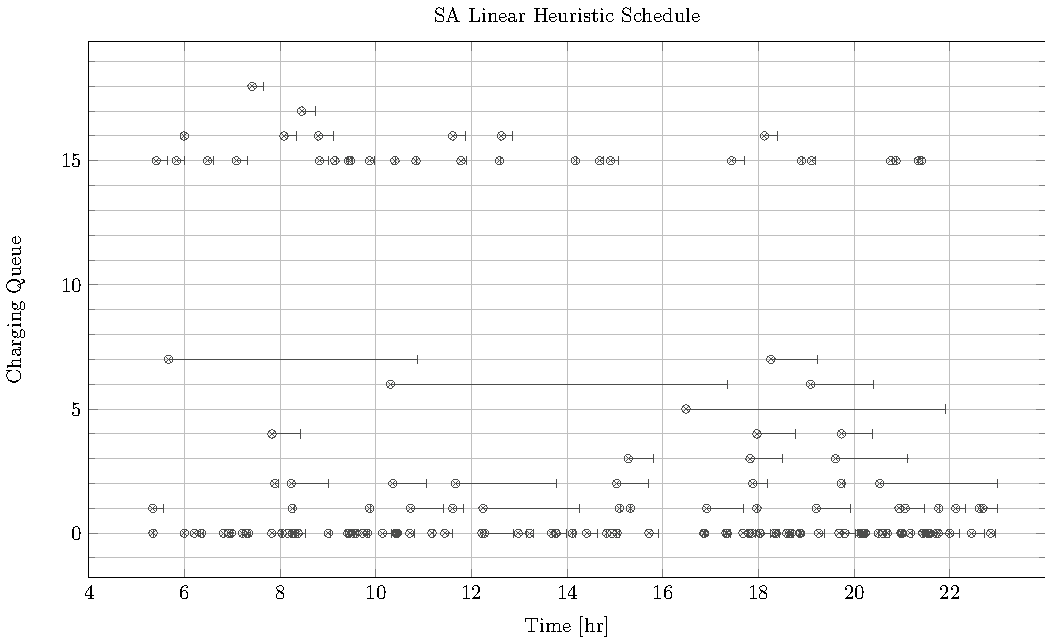
\includegraphics[width=0.7\textwidth]{img/sa-nonlinear/schedule-sa-heuristic}
\end{subfigure}
\end{figure}
\end{column}
\end{columns}
\end{frame}


\begin{frame}[label={sec:orgf6d5304}]{Mixed Integer Linear Programming}
\begin{align*}
\text{max }        &J = \sum_j c_j x_j + \sum_k d_k y_k&         &               \\
\text{subject to } &\sum_j a_{ij} x_j + \sum_k g_{ik} y_k \le b_i&  &(i = 1,2,...,m)\\
                  &x_j \ge 0&                              &(j = 1,2,...,n)\\
                  &y_k \in \mathbb{Z^+}&                   &(k = 1,2,...,n)\\
\end{align*}

\begin{itemize}
\item \(J\): Objective function
\item \(x_j \in \mathbb{R}\) and \(y_k \in \mathbb{Z}^+\): Decision Variables
\item \(c_j, d_k, a_{ij}, g_{ik}, b_i \in \mathbb{R}\): Parameters
\end{itemize}
\end{frame}


\begin{frame}[label={sec:org5a43d6b}]{}
\centering
\Huge Simulated Annealing
\end{frame}

\begin{frame}[label={sec:org0f6b185}]{Simulated Annealing\footnote{\url{https://en.wikipedia.org/wiki/Simulated\_annealing}}}
\begin{columns}
\begin{column}{0.5\columnwidth}
\begin{itemize}
\item A probabilistic technique for approximating the global optimum of a given function.
\item Often applied to problems that contain many local solutions
\item Three key components:
\begin{itemize}
\item Cooling Schedule
\item Acceptance Criteria
\item Generation Mechanisms
\end{itemize}
\end{itemize}
\end{column}

\begin{column}{0.5\columnwidth}
\centering
\animategraphics[width=0.9\linewidth]{10}{img/tsp/tsp-}{0}{87}
\end{column}
\end{columns}
\end{frame}

\begin{frame}[label={sec:orga607de6}]{Cooling Schedule}
\begin{columns}
\begin{column}{0.5\columnwidth}
\begin{itemize}
\item The cooling equation models the rate at which the temperature decreases over time in the SA process.
\item The temperature is high, SA encourages exploration. As the temperature decreases, exploitation is encouraged.
\end{itemize}
\end{column}

\begin{column}{0.5\columnwidth}
\begin{figure}[t!]
  \centering 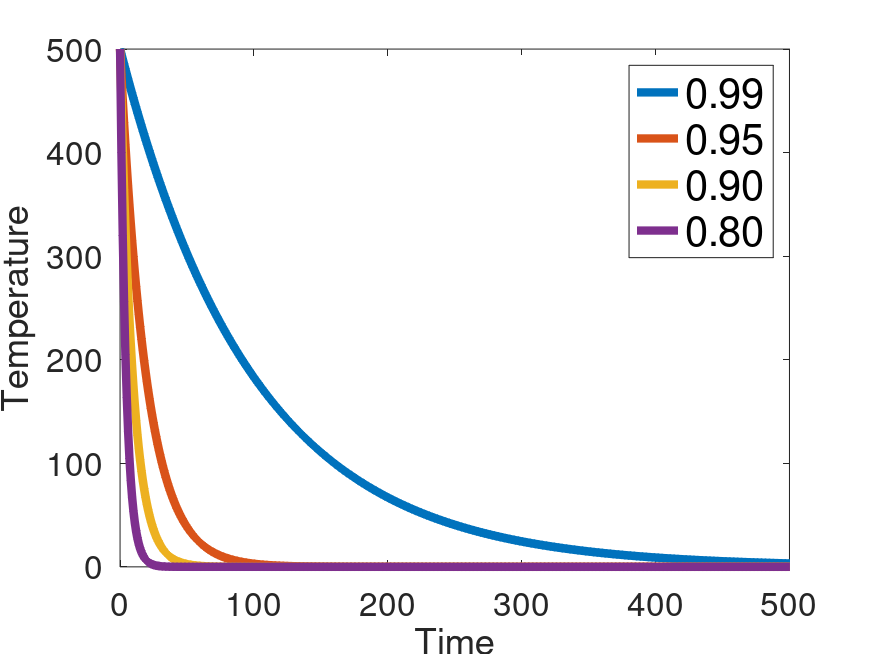
\includegraphics[width=0.9\textwidth]{img/geometric.png}
  \label{fig:geometric}
\end{figure}

\begin{equation*}
t_m = \beta t_{m-1}
\end{equation*}
\end{column}
\end{columns}
\end{frame}

\begin{frame}[label={sec:orgf2020b1}]{Acceptance Criteria\footnote{\url{https://en.wikipedia.org/wiki/Simulated\_annealing}}}
\begin{equation*}
\label{eq:candaccept}
f(\mathbb{I},\bar{\mathbb{I}},t_m) =
\begin{cases}
  1                   & \Delta E > 0 \\
  e^{- \frac{\Delta E}{t_m}} & \text{otherwise}
\end{cases}
\end{equation*}

\begin{columns}
\begin{column}{0.7\columnwidth}
\centering
\animategraphics[width=\linewidth]{10}{img/sa-visual/sa-}{90}{274}
\end{column}

\begin{column}{0.3\columnwidth}
\begin{figure}[t!]
  \centering 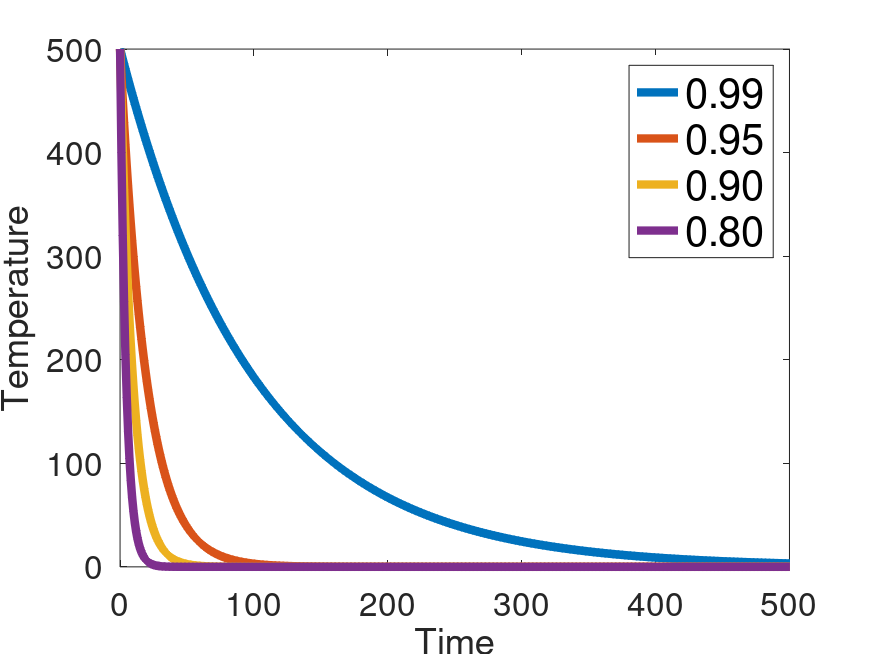
\includegraphics[width=\textwidth]{img/geometric.png}
  \label{fig:geometric}
\end{figure}
\end{column}
\end{columns}
\end{frame}

\begin{frame}[label={sec:org2e5b99e}]{Generation Mechanisms - Primitive Functions}
\begin{columns}
\begin{column}{0.4\columnwidth}
\begin{itemize}
\item New Visit: Move a bus from a wait queue to charge queue
\item Slide Visit: Change the charge duration of a visit
\item New Charger: Move a visit to a new charger
\item Wait: Move a visit to its idle queue
\item New Window: Execute Wait then New Visit primitives
\end{itemize}
\end{column}

\begin{column}{0.6\columnwidth}
\begin{figure}
    \centering
    \scalebox{0.4}{
      \centering
        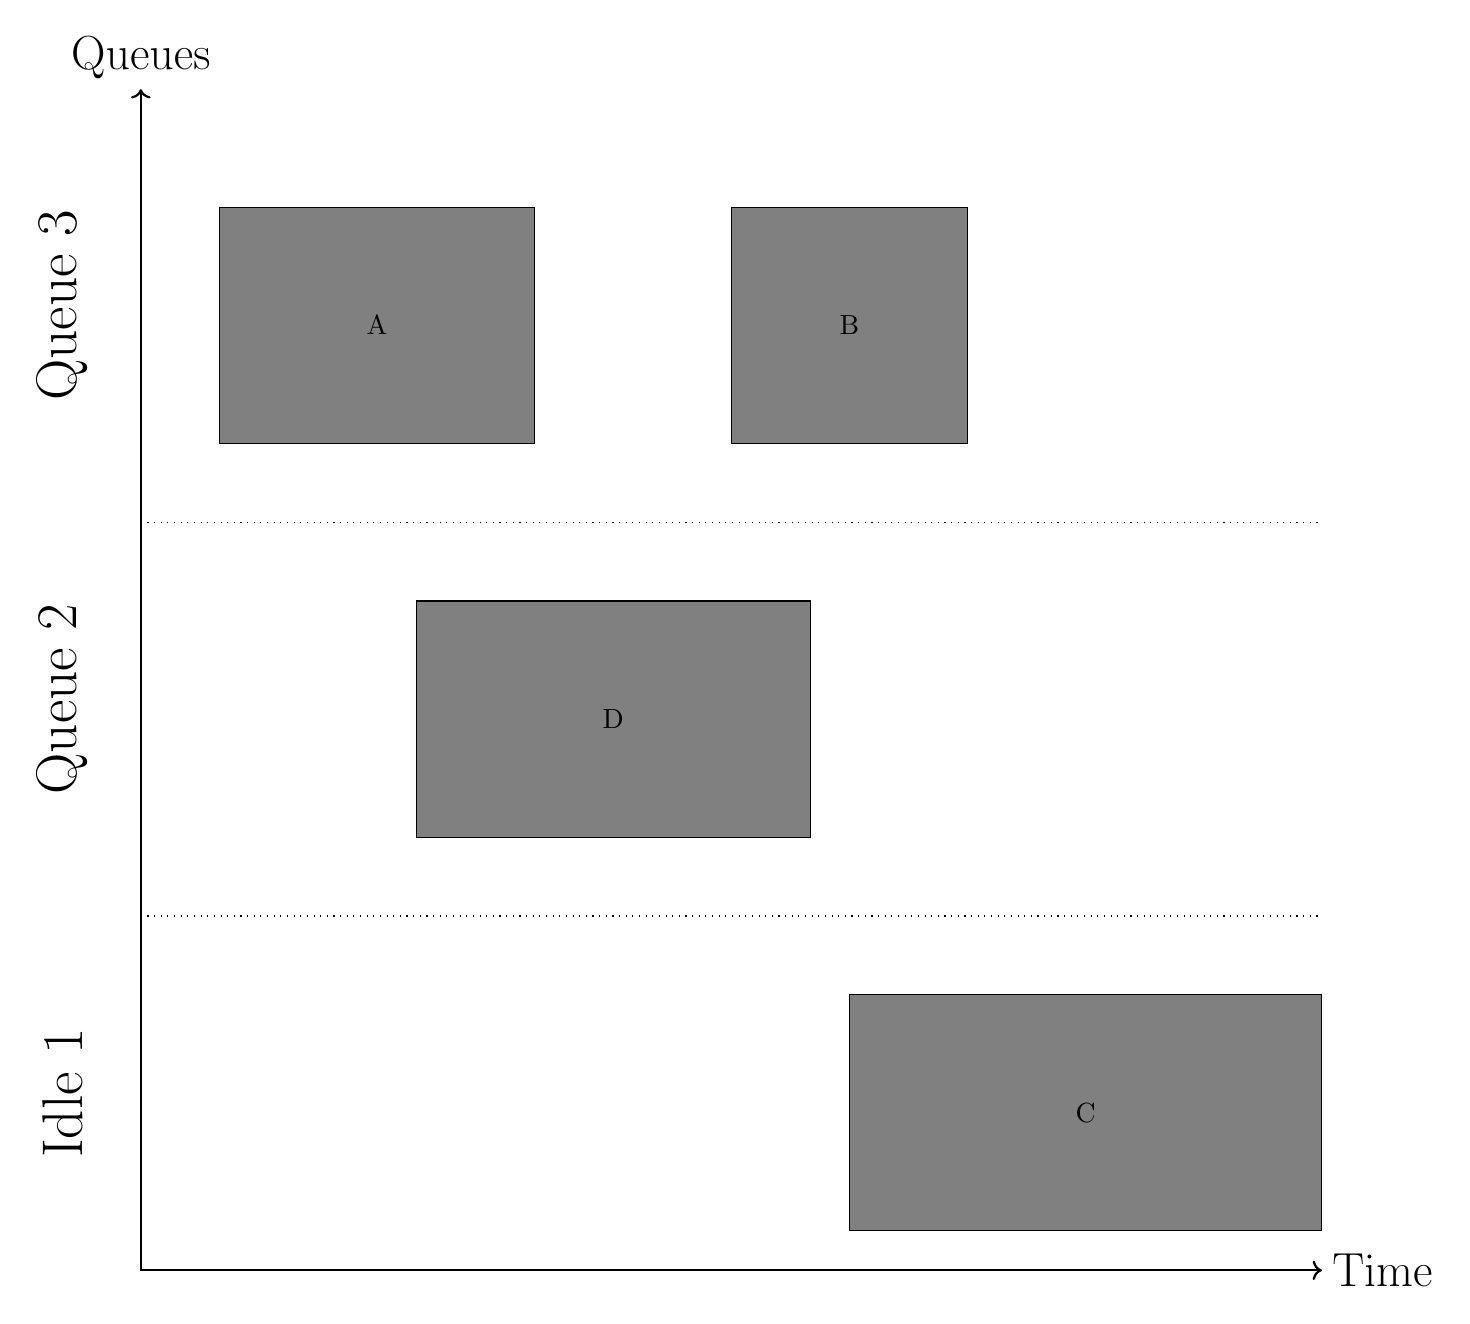
\begin{tikzpicture}
          % Variables
          \def \arrx   {2.0}
          \def \initx  {3.5}
          \def \endx   {8.5}
          \def \depx   {10.0}
          \def \yshift {5}

          % Axis
          \draw [thick,<->] (0,15) node[above]{\LARGE Queues} -- (0,0) -- (15,0) node[right]{\LARGE Time};

          % Rectangles
          \node[rectangle, draw, fill=gray, minimum width=4cm, minimum height = 3cm] at (3,12) {A};
          \node[rectangle, draw, fill=gray, minimum width=3cm, minimum height = 3cm] at (9,12) {B};
          \node[rectangle, draw, fill=gray, minimum width=5cm, minimum height = 3cm] at (6,7) {D};
          \node[rectangle, draw, fill=gray, minimum width=6cm, minimum height = 3cm] at (12,2) {C};

          % Y-axis labels
          \node[rotate=90] at (-1, 2.25) {\huge Idle 1};
          \node[rotate=90] at (-1, 7.25) {\huge Queue 2};
          \node[rotate=90] at (-1, 12.25) {\huge Queue 3};

          % Horizontal lines
          \draw[dotted] (0, 4.5) -- (15, 4.5);
          \draw[dotted] (0, 9.5) -- (15, 9.5);

        \end{tikzpicture}
      }
      \label{fig:spacial-and-temporal-constr}
\end{figure}
\end{column}
\end{columns}
\end{frame}

\begin{frame}[label={sec:org47e0b52}]{Generation Mechanisms - Wrapper Functions}
\begin{columns}
\begin{column}{0.4\columnwidth}
\begin{itemize}
\item Charge Schedule Generation: Iterate through each visit and execute New Visit
\item Perturb Schedule: Randomly execute one of the primitives with a weighted distribution
\end{itemize}
\end{column}

\begin{column}{0.6\columnwidth}
\begin{figure}
    \centering
      \centering
    \scalebox{0.4}{
        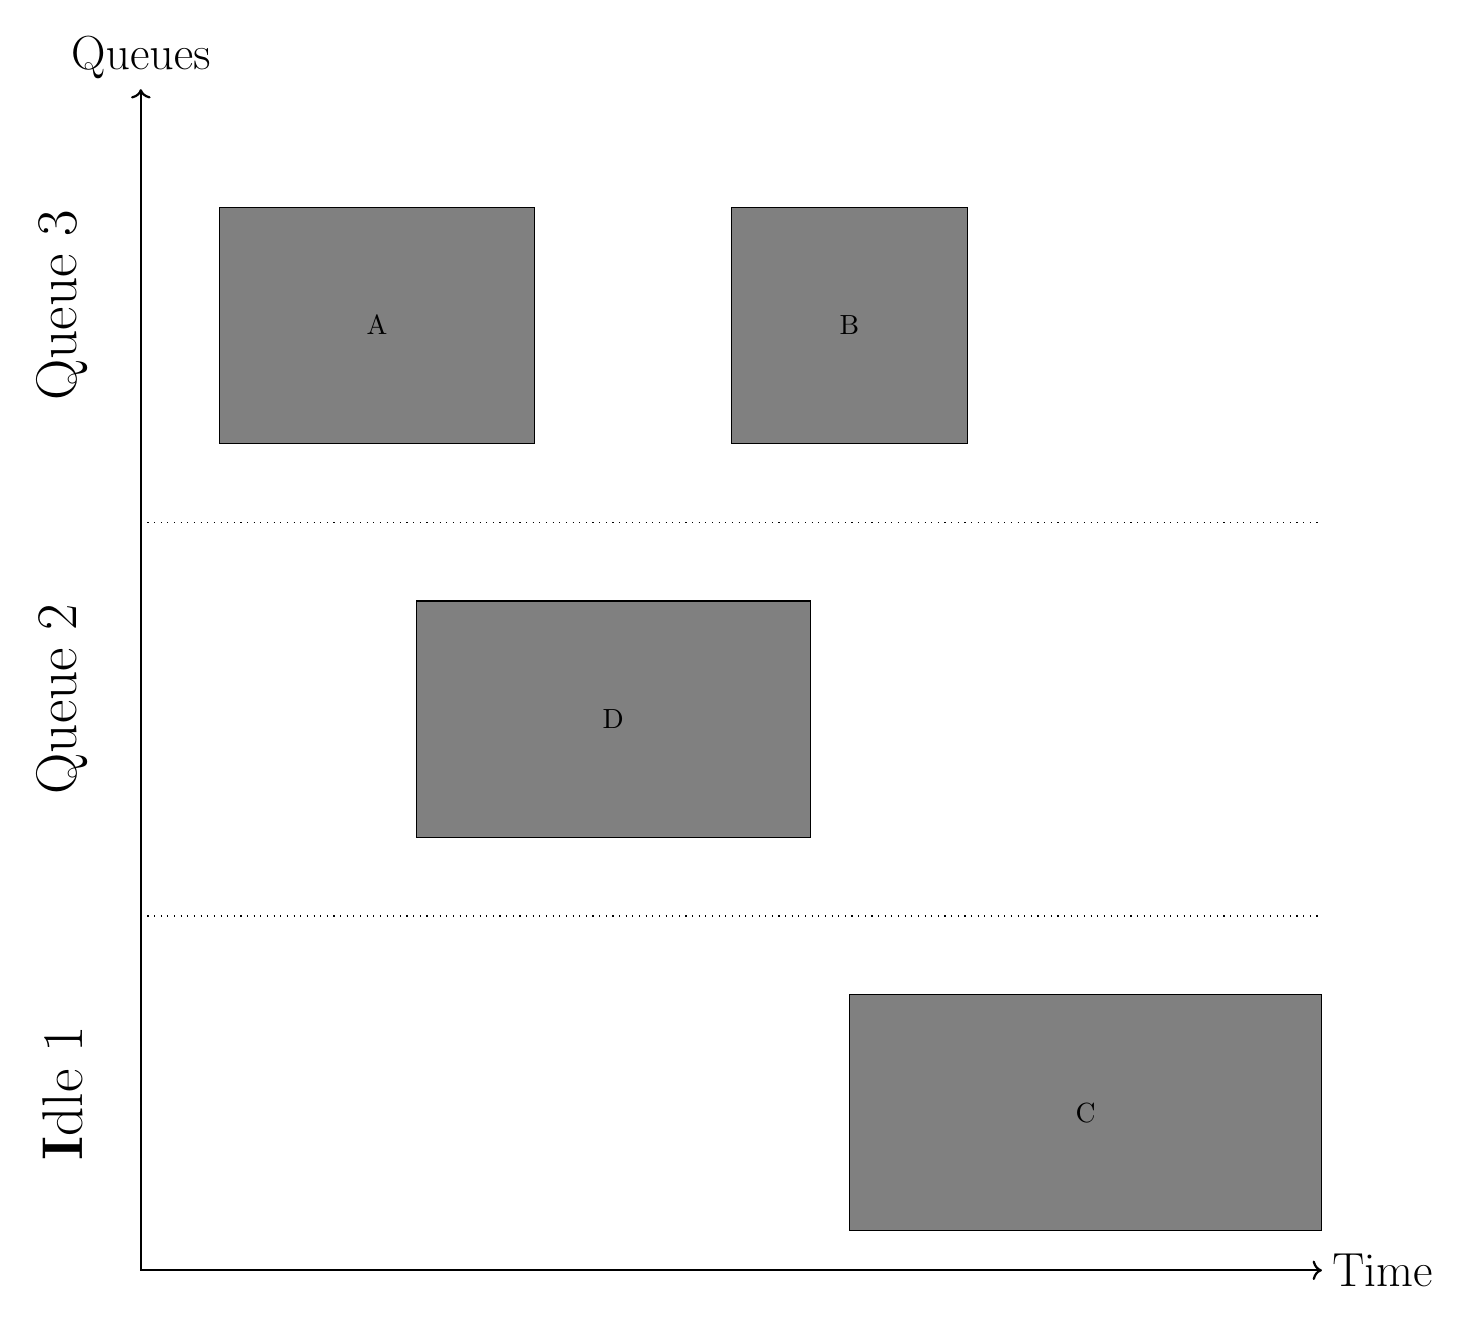
\begin{tikzpicture}
          % Variables
          \def \arrx   {2.0}
          \def \initx  {3.5}
          \def \endx   {8.5}
          \def \depx   {10.0}
          \def \yshift {5}

          % Axis
          \draw [thick,<->] (0,15) node[above]{\LARGE Queues} -- (0,0) -- (15,0) node[right]{\LARGE Time};

          % Rectangles
          \node[rectangle, draw, fill=gray, minimum width=4cm, minimum height = 3cm] at (3,12) {A};
          \node[rectangle, draw, fill=gray, minimum width=3cm, minimum height = 3cm] at (9,12) {B};
          \node[rectangle, draw, fill=gray, minimum width=5cm, minimum height = 3cm] at (6,7) {D};
          \node[rectangle, draw, fill=gray, minimum width=6cm, minimum height = 3cm] at (12,2) {C};

          % Y-axis labels
          \node[rotate=90] at (-1, 2.25) {\huge \textbf Idle 1};
          \node[rotate=90] at (-1, 7.25) {\huge Queue 2};
          \node[rotate=90] at (-1, 12.25) {\huge Queue 3};

          % Horizontal lines
          \draw[dotted] (0, 4.5) -- (15, 4.5);
          \draw[dotted] (0, 9.5) -- (15, 9.5);

        \end{tikzpicture}
      }
      \label{fig:spacial-and-temporal-constr}
\end{figure}
\end{column}
\end{columns}
\end{frame}

\begin{frame}[label={sec:org0f522da}]{New Visit}
\begin{algorithm}[H]
  \scriptsize
  \caption{New visit algorithm}
  \label{alg:new-visit}
  \LinesNumbered
  \TitleOfAlgo{New Visit}
  \KwIn{$\Sol$}
  \KwOut{$\bar{\Sol}$}

  \SetKwFunction{Union}{Union}
  \SetKwFunction{findFreeTime}{findFreeTime}

  \Begin
    {
      $i \leftarrow \Sol_{i}$\tcc*{Extract visit index}
      $a \leftarrow \I_{i.a}$\tcc*{Extract the arrivial time for visit $i$}
      $e \leftarrow \I_{i.e}$\tcc*{Extract the departure time for visit $i$}
      $q \leftarrow \I_{i.q}$\tcc*{Extract the current charge queue for visit $i$}
      $\bar{q} \leftarrow \mathcal{U}_{Q}$\tcc*{Select a random charging queue with a uniform distribution}
      $C \leftarrow \mathcal{U}_{\C_q}$\tcc*{Select a random time slice from $\C_q$}

      \If(\tcc*[f]{If there is time available in $C_q^j$}){($\bar{C}, \bar{u}, \bar{d}$) $\leftarrow$ \findFreeTime{$C, i, q, a, e$} $\not\in \varnothing$}
         {
           \Return{($i, (\bar{q},\bar{u},\bar{d}),\bar{C}$)}\tcc*[f]{Return visit}
         }

         \Return{($\varnothing$)}\tcc*{Return nothing}
    }
\end{algorithm}
\end{frame}

\begin{frame}[label={sec:org686f100}]{Slide Visit}
\begin{algorithm}[H]
  \scriptsize
  \caption{Slide Visit Algorithm} \label{alg:slide-visit}
  \LinesNumbered
  \TitleOfAlgo{Slide Visit}
  \KwIn{$\Sol$}
  \KwOut{$\bar{\Sol}$}

    \SetKwFunction{Purge}{Purge}

    \Begin
    {
      $(i, \I, \bar{\C}) \leftarrow$\Purge{$\Sol$}\tcc*{Purge visit $i$ from charger availibility matrix}
      $C \leftarrow \bar{C}_{i.q_i}$\tcc*{Get the time availability of the purged visit}

      \tcc{If there is time available in $C$}
      \If{($\bar{C}, \bar{u}, \bar{d}$) $\leftarrow$ \findFreeTime{$C$, $\Sol_i$, $\I_q$, $\I_{i.a}, \I_{i.e}$} $\not\in \varnothing$}
      {
        \Return{($i, \I, (\I_{i.q_i},\bar{u},\bar{d}),\bar{C}$)}\tcc*[f]{Return updated visit}
      }

        \Return{($\varnothing$)}\tcc*{Return nothing}
    }
  \end{algorithm}
\end{frame}

\begin{frame}[label={sec:orga0d45e9}]{New Charger}
\begin{algorithm}[H]
  \scriptsize
  \caption{New Charger Algorithm} \label{alg:new-charger} \LinesNumbered \TitleOfAlgo{New Charger} \KwIn{$\Sol$}
  \KwOut{$\bar{\Sol}$}

    \SetKwFunction{Purge}{Purge}

    \Begin
    {
      $(i, \I, \bar{\C}) \leftarrow$\Purge{$\Sol$}\tcc*{Purge visit $i$ from charger availibility matrix}
      $q \leftarrow \mathcal{U}_{Q}$\tcc*{Select a random charging queue with a uniform distribution}

      \If(\tcc*[f]{If there is time available in $C_{q}$}){($\bar{C}, \bar{u}, \bar{d}$) $\leftarrow$ \findFreeTime{$\bar{\C}_{i.q}$, $\Sol_i$, $\I_q$, $\I_{i.a}, \I_{i.e}$} $\not\in \varnothing$}
      {
        \tcc{Return visit, note $u$ and $d$ are the original inital/final charge times.}
        \Return{($i, \I, (q,\I_{i.u}, \I_{i.d}),\bar{\C}$)}
      }

      \Return{($\varnothing$)}\tcc*{Return nothing}
    }
  \end{algorithm}
\end{frame}

\begin{frame}[label={sec:org510ffd0}]{Wait}
\begin{algorithm}[H]
\scriptsize
\caption{Wait algorithm} \label{alg:wait}
    \LinesNumbered
    \TitleOfAlgo{Wait}
    \KwIn{$\Sol$}
    \KwOut{$\bar{\Sol}$}

    \SetKwFunction{Purge}{Purge}

    \Begin
    {
      $(i, \I, \bar{\C}) \leftarrow$\Purge{$\Sol$}\tcc*{Purge visit $i$ from charger availibility matrix}
      $\bar{\C}'_{\I_{i.\Gamma_i}} \leftarrow \C' \cup \{[\I_{i.a}, \I_{i.e}]\}$\tcc*{Update the charger availability matrix for wait queue $\bar{\C}_{i.q_i}$}
      \Return{$(i, \I, (\I_{i.b}, \I_{i.a}, \I_{i.e}), \bar{\C})$}\tcc*[f]{Return visit}
    }
  \end{algorithm}
\end{frame}

\begin{frame}[label={sec:orga6cd612}]{New Window}
\begin{algorithm}[H]
  \scriptsize
  \caption{New window algorithm} \label{alg:new-window}
  \LinesNumbered
  \TitleOfAlgo{New Window}
  \KwIn{$\Sol$}
  \KwOut{$\bar{\Sol}$}

  \SetKwFunction{NewVisit}{NewVisit}
  \SetKwFunction{Wait}{Wait}

  \Begin
  {
    $\bar{\Sol} \leftarrow$\Wait{$\Sol$}\tcc*{Assign visit to its respective idle queue}
    \If(\tcc*[f]{Add visit $i$ back in randomly})
       {
         $\bar{\bar{\Sol}} \leftarrow$ \NewVisit{$\bar{\Sol}$} $\not\in \varnothing$
       }
       {
         \Return{$\bar{\bar{\Sol}}$} \tcc*[f]{Return visit}
       }

       \Return{($\varnothing$)}\tcc*{Return nothing}
  }
\end{algorithm}
\end{frame}

\begin{frame}[label={sec:org0db87e7}]{Charge Schedule Generation}
\begin{algorithm}[H]
\scriptsize
\caption{Charge schedule generation algorithm} \label{alg:charge-schedule-generation}
    \LinesNumbered
    \TitleOfAlgo{Candidate Solution Generator}
    \KwIn{$\Sol$}
    \KwOut{$\bar{\Sol}$}

    \SetKwFunction{NewVisit}{NewVisit}

    \Begin
    {
        \tcc{Select an unscheduled BEB visit from a randomly indexed set of visits}
        \ForEach {$\I_i \in \I$}
        {
            ($i, \bar{\I}$, $\bar{\C}$) $\leftarrow$ \NewVisit{($\I_i$, $\I$, $\C$)}\tcc*{Assign the bus to a charger}
        }
            \Return{($0, \bar{\I}$, $\bar{\C}$)}
    }
  \end{algorithm}
\end{frame}

\begin{frame}[label={sec:org168fd77}]{Charge Schedule Perturbation}
\begin{center}
\scalebox{0.65}{
\begin{minipage}{1.5\linewidth}
\begin{algorithm}[H]
\scriptsize
\caption{Perturb schedule algorithm} \label{alg:perturb-schedule}

    \LinesNumbered
    \TitleOfAlgo{Perturb Schedule}
    \KwIn{$\Sol$}
    \KwOut{$\bar{\Sol}$}

    \SetKwFunction{PGF}{PGF}

    \Begin
    {
        $p \leftarrow [false; n_A]$\tcc*{Create vector to track priority routes}
        $y^i \leftarrow [1.0; n_V]$\tcc*{Create weight vector for index selection}
        \tcc{Loop through the visits in reverse order}
        \ForEach{$\I_i \leftarrow \I_{|\I|} \text{ TO } \I_{1}$}
        {
            \tcc{If the current visit is part of a priority route}
            \If{$p_{\I_{i.b}} = true$}{$y^i_{\I_i} = y^i_{\I_{i.\xi}}$\;}
            \tcc{Else if the current visit's SOC does below the allowed threshold}
            \ElseIf{$\I_{i.\eta} \le \nu_{\I_{i.b}} \kappa_{\I_{i.b}}$}{
                $p_{\I_{i.b}} = true$\tcc*{Indicate the current BEB's routes are to be prioritized}
                $y^i_{\I_i} = \kappa_{\I_{i.b}} (\nu_{\I_{i.b}}\kappa_{\I_{i.b}} - \I_{i.\eta})$\tcc*{Calculate the weight of the current visit}
            }
        }
        $\I_i\leftarrow\; \W^{y^i}_{\I}$\tcc*{Select an index with a weighted distribution}
        $i \leftarrow\; \I_i$\tcc*{Extract visit index}
        $y^p \leftarrow [y^p_1, y^p_2, ...]$\tcc*{Define the weight of each primitive generator}
        $PGF \leftarrow\; \W^{y^p}_{[1,n_G]}$\tcc*{Select a generator function with weighted distribution}
        $\bar{\Sol} \leftarrow$ \PGF{($i$, $\I$, $\C$)}\tcc*{Excecute the generator function}
        \Return{($0, \bar{\I}$, $\bar{\C}$)}
    }
\end{algorithm}
\end{minipage}}
\end{center}
\end{frame}

\begin{frame}[label={sec:org6529144}]{}
\centering
\Huge Thesis Results
\end{frame}

\begin{frame}[label={sec:org56e93fd}]{Parameters}
\begin{center}
\begin{tabular}{lrr}
\alert{Model} & \alert{Execution Time} [s] & \alert{Iteration} [s]\\[0pt]
\hline
MILP & 3600 & N/A\\[0pt]
Quick & 2275.25 & 0.25\\[0pt]
Heuristic & 3640.4 & 0.4\\[0pt]
\end{tabular}
\end{center}

\begin{columns}
\begin{column}{0.5\columnwidth}
\begin{itemize}
\item \(T_0 = 99999\)
\item \(\beta = 0.999\)
\end{itemize}
\end{column}
\begin{column}{0.5\columnwidth}
\begin{itemize}
\item \(|t| = 3797\)
\item \(n_K = 500\)
\end{itemize}
\end{column}
\end{columns}
\end{frame}

\begin{frame}[label={sec:org4718426}]{Schedule}
\begin{columns}
\begin{column}{0.5\columnwidth}
\begin{figure}[htpb]
\centering
    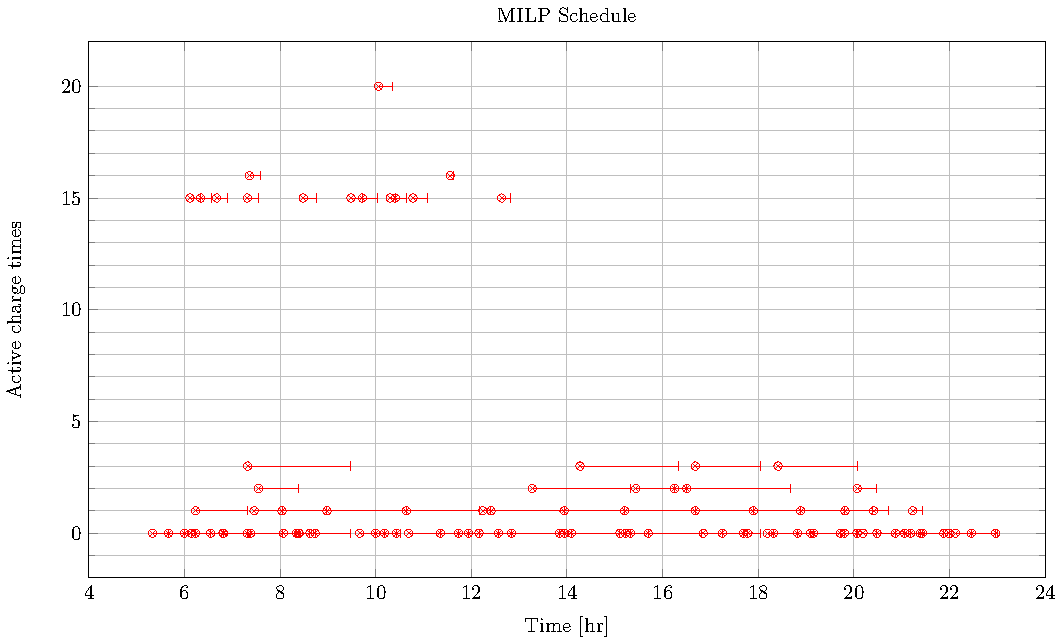
\includegraphics[width=\textwidth]{img/sa-pap-paper-bad/schedule-milp}
\end{figure}
\end{column}
\begin{column}{0.5\columnwidth}
\begin{figure}[htpb]
\centering
    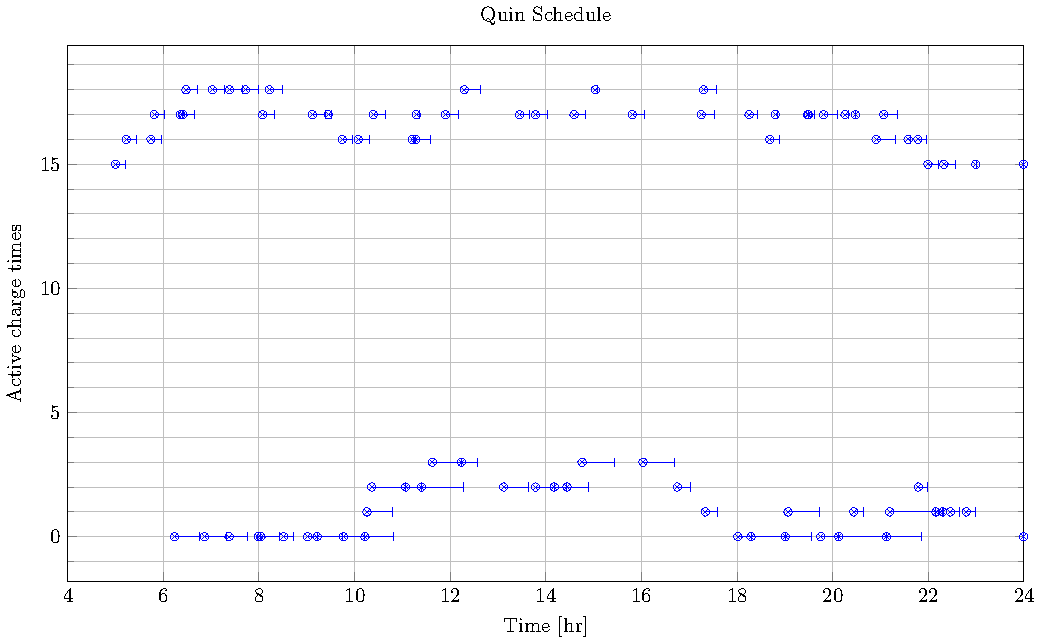
\includegraphics[width=\textwidth]{img/sa-pap-paper-bad/schedule-quinn}
\end{figure}
\end{column}
\end{columns}
\end{frame}

\begin{frame}[label={sec:org40b17a5}]{Schedule}
\begin{columns}
\begin{column}{0.5\columnwidth}
\begin{figure}[htpb]
\centering
    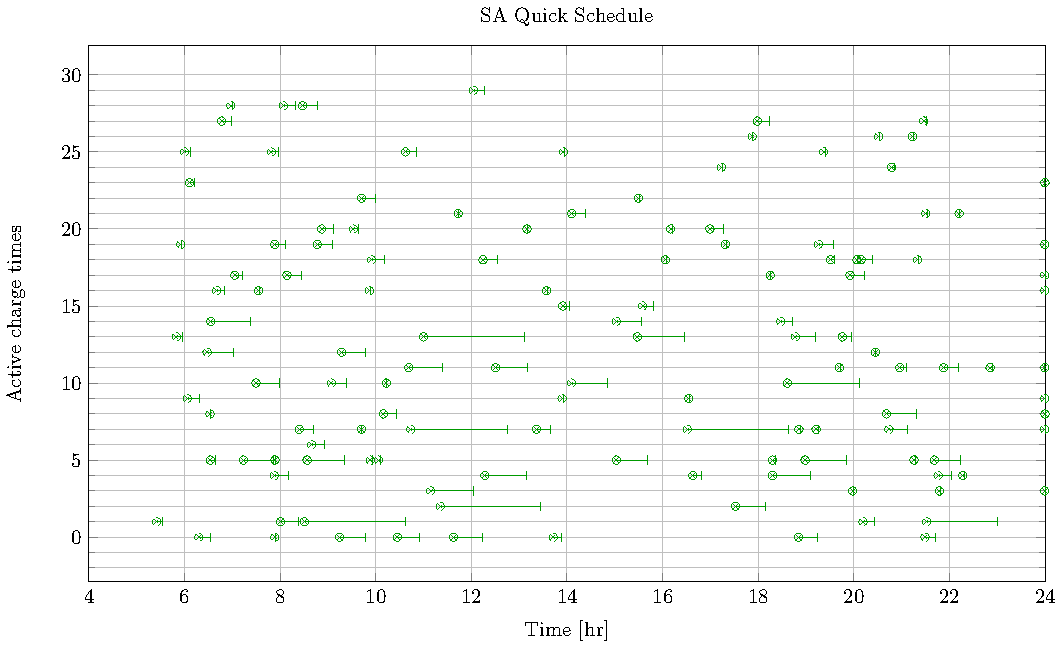
\includegraphics[width=\textwidth]{img/sa-pap-paper-bad/schedule-sa-quick}
\end{figure}
\end{column}

\begin{column}{0.5\columnwidth}
\begin{figure}[htpb]
\centering
    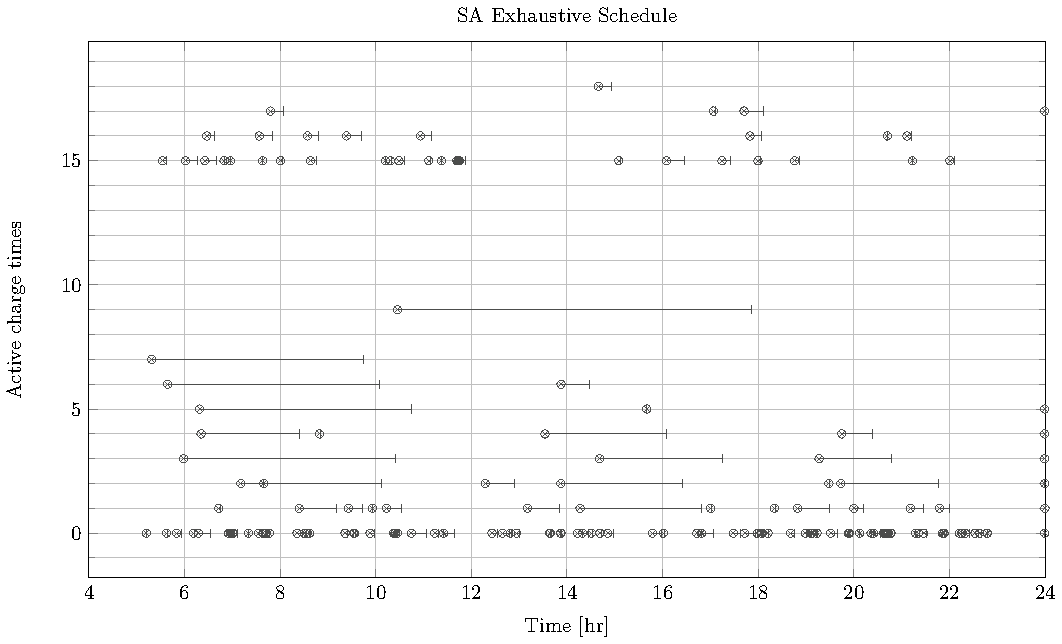
\includegraphics[width=\textwidth]{img/sa-pap-paper-bad/schedule-sa-heuristic}
\end{figure}
\end{column}
\end{columns}
\end{frame}

\begin{frame}[label={sec:orgdb153e9}]{Power}
\begin{columns}
\begin{column}{0.5\columnwidth}
\begin{figure}[htpb]
\centering
    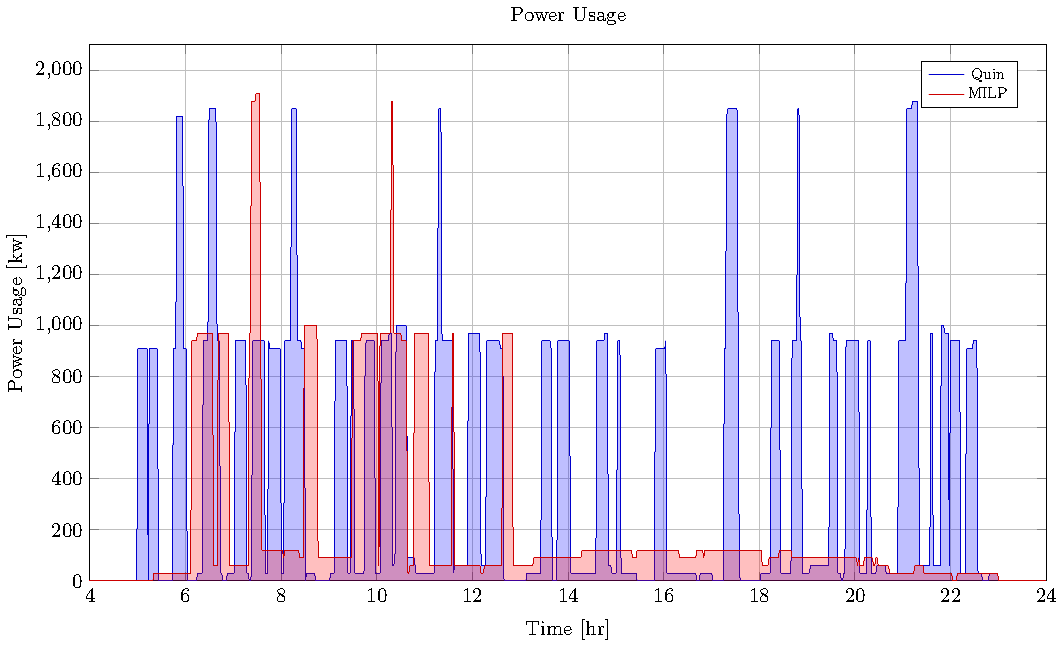
\includegraphics[width=\textwidth]{img/sa-pap-paper-bad/power-milp-qin}
\end{figure}
\end{column}

\begin{column}{0.5\columnwidth}
\begin{figure}[htpb]
\centering
    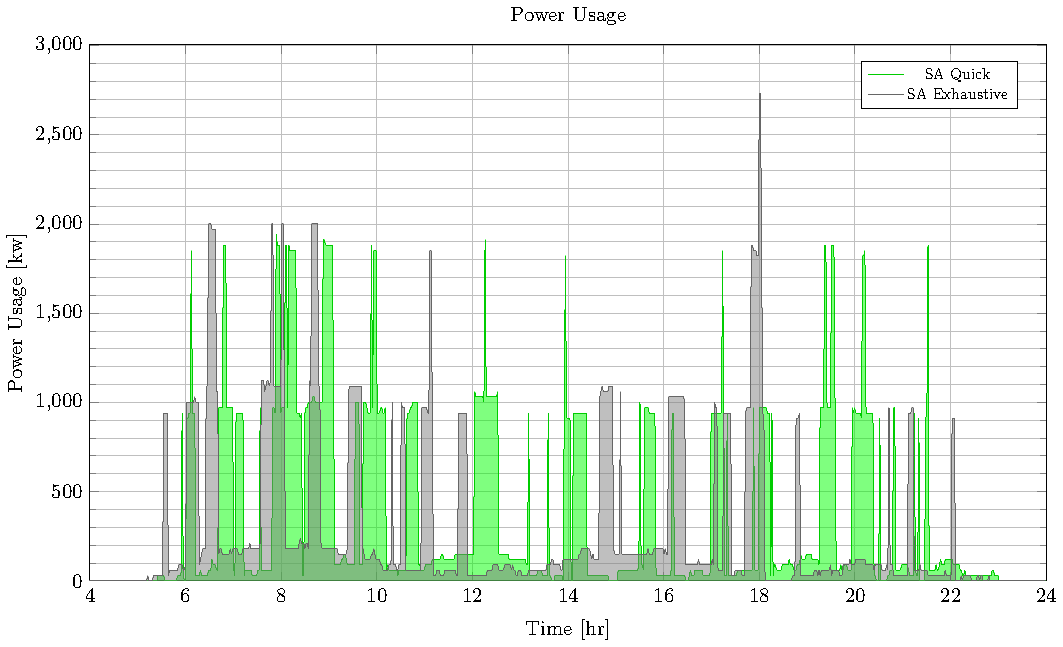
\includegraphics[width=\textwidth]{img/sa-pap-paper-bad/power-sa}
\end{figure}
\end{column}
\end{columns}
\end{frame}
\begin{frame}[label={sec:org06ec095}]{Energy}
\begin{figure}[htpb]
\centering
    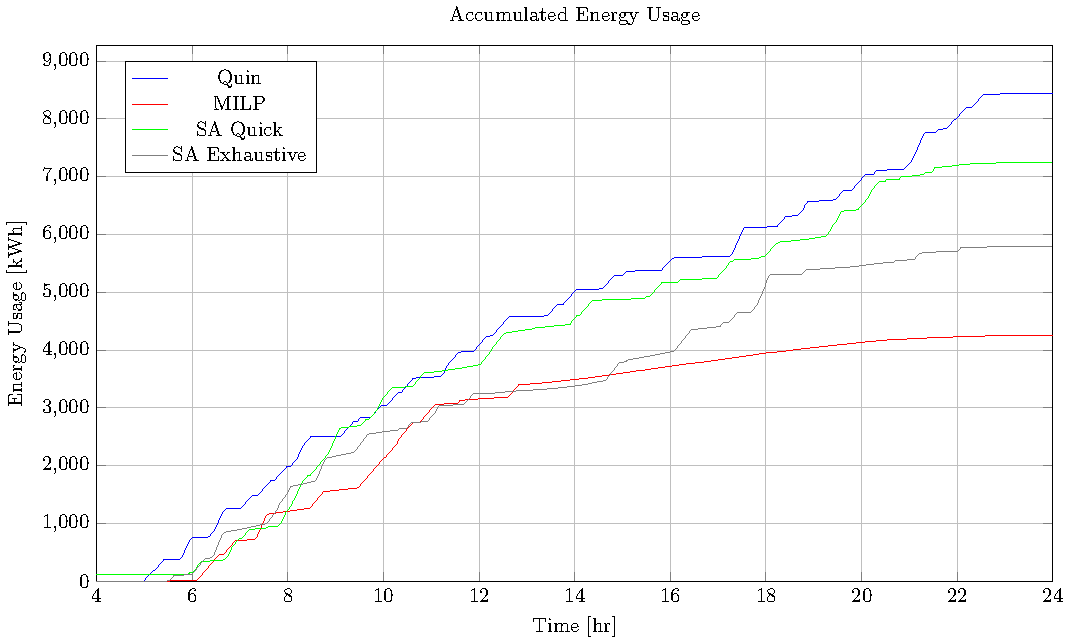
\includegraphics[width=0.6\textwidth]{img/sa-pap-paper-bad/energy}
\end{figure}
\end{frame}

\begin{frame}[label={sec:orgf47a263}]{How To Resolve This Problem?}
\begin{columns}
\begin{column}{0.5\columnwidth}
\begin{figure}[htpb]
\centering
    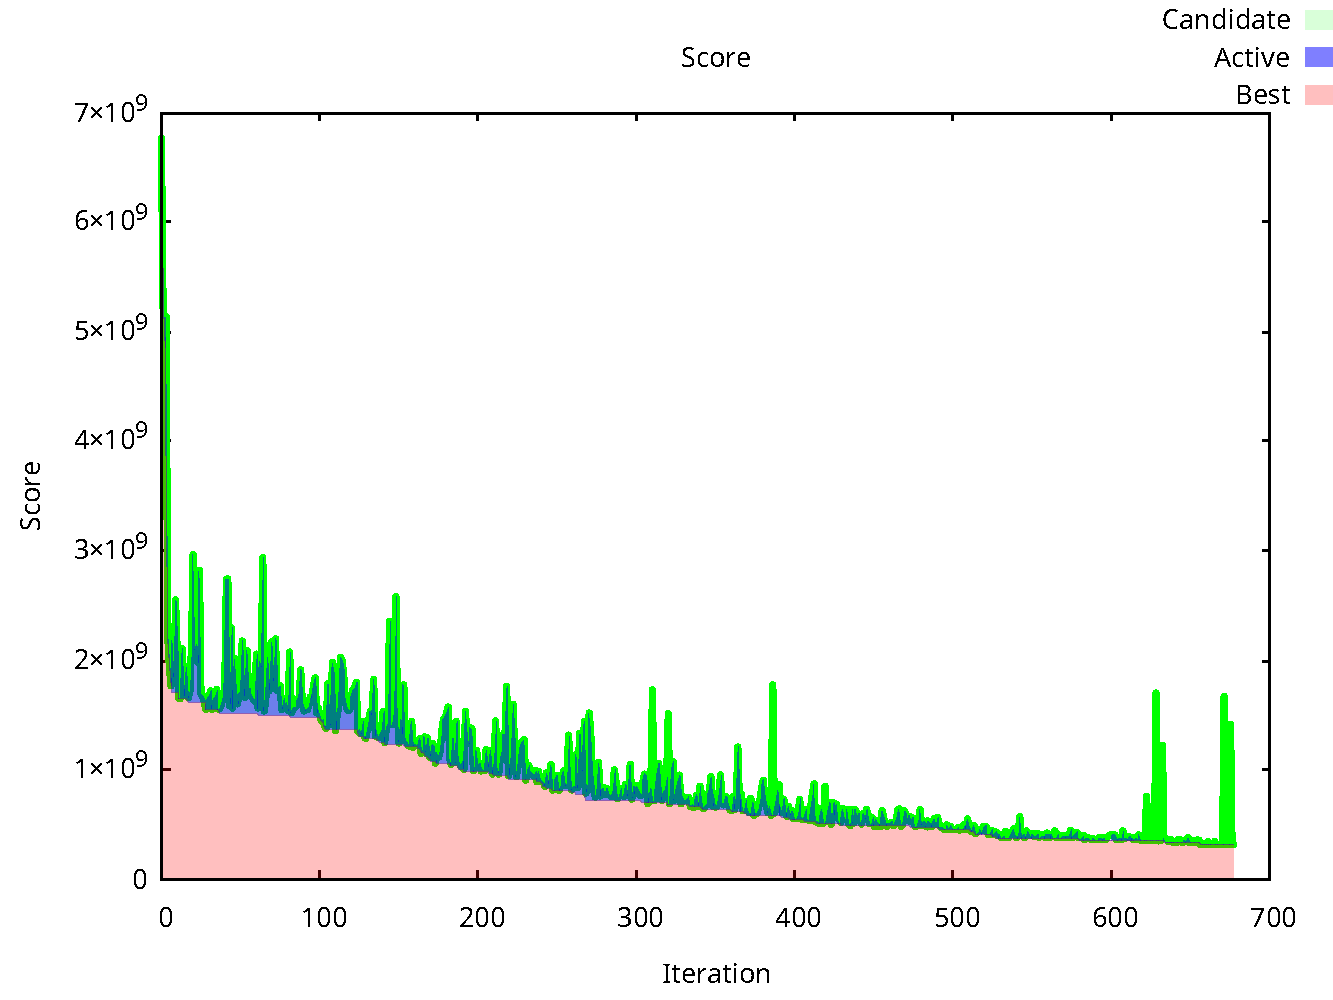
\includegraphics[width=\textwidth]{img/score-convergence}
\end{figure}

\begin{itemize}
\item Reverse search and weight the visit indices
\item Be more aggressive in exploiting the best solution
\end{itemize}
\end{column}

\begin{column}{0.5\columnwidth}
\begin{figure}[htpb]
\centering
    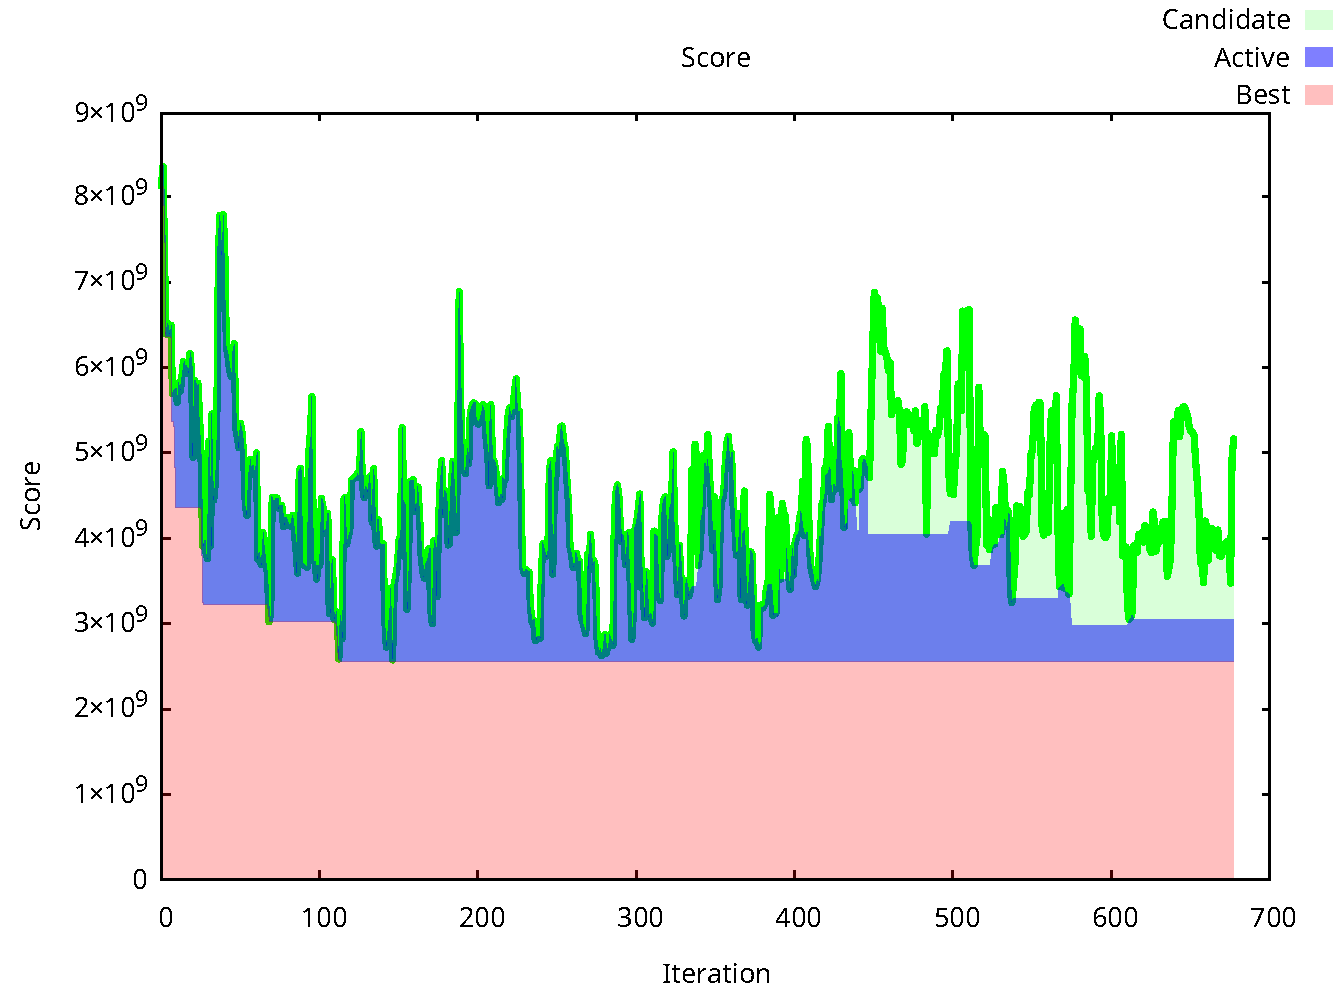
\includegraphics[width=\textwidth]{img/score-diverge}
\end{figure}

\begin{itemize}
\item Candidate solutions diverge
\item Hard time handling ``difficult'' routes
\end{itemize}
\end{column}
\end{columns}
\end{frame}

\begin{frame}[label={sec:org8257739}]{Score Convergence Comparison}
\begin{columns}
\begin{column}{0.5\columnwidth}
\begin{center}
Before Fix
\end{center}

\begin{figure}[htpb]
\centering
    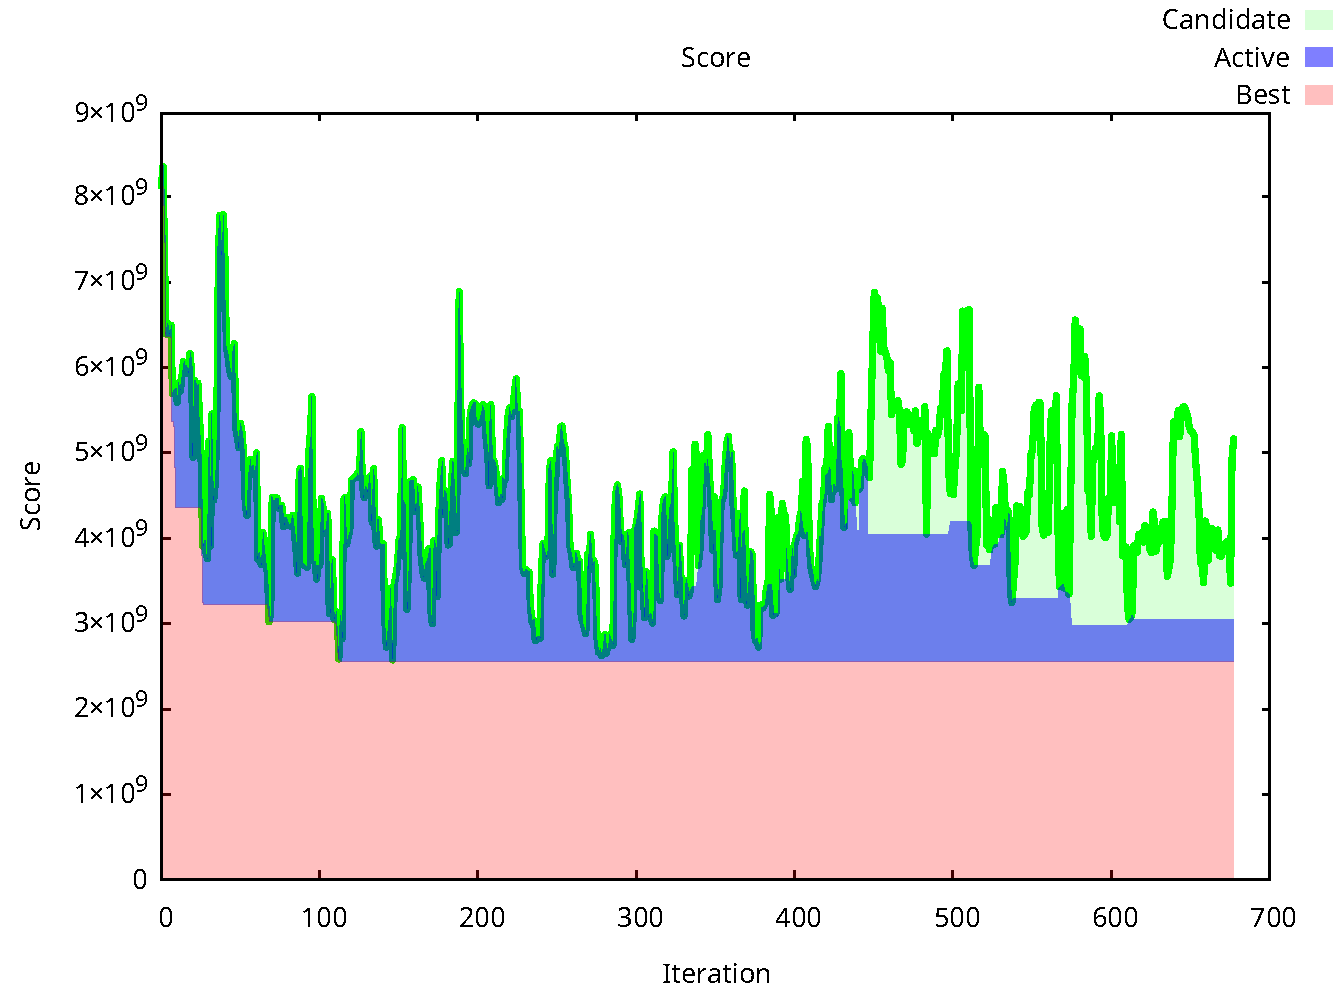
\includegraphics[width=\textwidth]{img/score-diverge}
\end{figure}
\end{column}

\begin{column}{0.5\columnwidth}
\begin{center}
After Fix
\end{center}

\begin{figure}[htpb]
\centering
    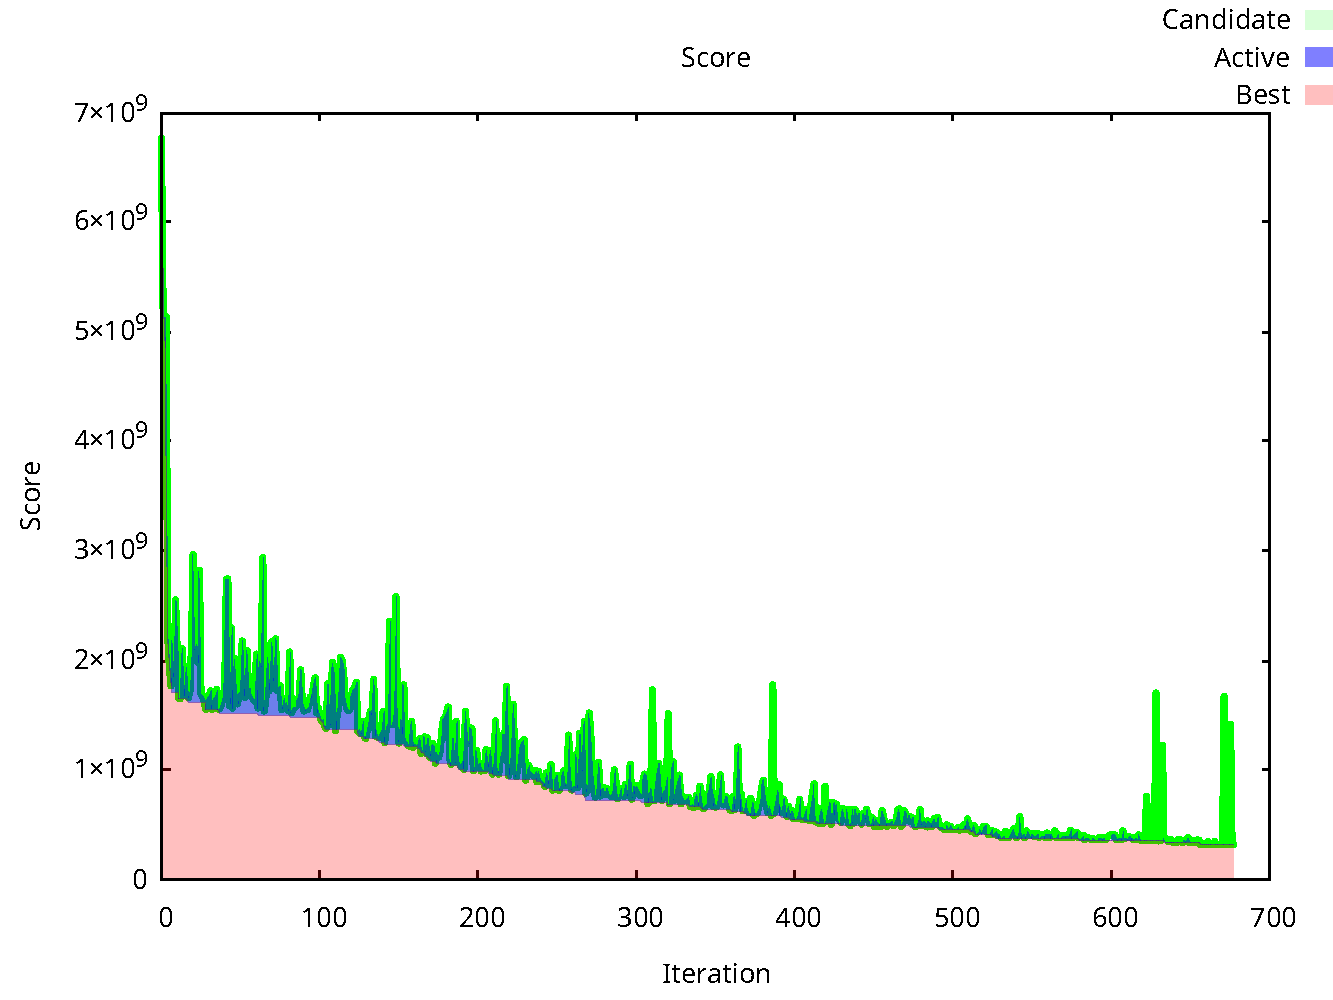
\includegraphics[width=\textwidth]{img/score-convergence}
\end{figure}
\end{column}
\end{columns}
\end{frame}


\begin{frame}[label={sec:org676b085}]{References}
\bibliographystyle{plain}
\bibliography{/home/alex/Documents/citation-database/lit-ref,/home/alex/Documents/citation-database/lib-ref}
\end{frame}
\end{document}
